% !Mode:: "TeX:UTF-8"
% !TEX encoding = UTF-8 Unicode

%----------------------------------------------------------------------------------------
% 机器翻译:基础与模型
% Machine Translation: Foundations and Models
%
% Copyright 2020
% 肖桐(xiaotong@mail.neu.edu.cn) 朱靖波 (zhujingbo@mail.neu.edu.cn)
%----------------------------------------------------------------------------------------

%----------------------------------------------------------------------------------------
%    CONFIGURATIONS
%----------------------------------------------------------------------------------------

\renewcommand\figurename{图}%将figure改为图
\renewcommand\tablename{表}%将figure改为图
\chapterimage{fig-NEU-10.jpg} % Chapter heading image

%----------------------------------------------------------------------------------------
%	CHAPTER 10
%----------------------------------------------------------------------------------------

\chapter{基于循环神经网络的模型}

\parinterval {\small\bfnew{神经机器翻译}} \index{神经机器翻译}(Neural Machine Translation)\index{Neural Machine Translation}是机器翻译的前沿方法。近几年,随着深度学习技术的发展和在各领域中的深入应用,基于端到端表示学习的方法正在改变着我们处理自然语言的方式,神经机器翻译在这种趋势下应运而生。一方面,神经机器翻译仍然延续着统计建模和基于数据驱动的思想,因此在基本问题的定义上与前人的研究是一致的;另一方面,神经机器翻译脱离了统计机器翻译中对隐含翻译结构的假设,同时使用分布式表示来对文字序列进行建模,这使得它可以从一个全新的视角看待翻译问题。现在,神经机器翻译已经成为了机器翻译研究及应用的热点,译文质量得到了巨大的提升。

\parinterval 本章将介绍神经机器翻译中的一种基础模型\ \dash \ 基于循环神经网络的模型。该模型是神经机器翻译中最早被成功应用的模型之一。基于这个模型框架,研究人员进行了大量的探索和改进工作,包括使用LSTM等循环单元结构、引入注意力机制等。这些内容都会在本章进行讨论。

%----------------------------------------------------------------------------------------
%    NEW SECTION  10.1
%----------------------------------------------------------------------------------------
\section{神经机器翻译的发展简史}

\parinterval 纵观机器翻译的发展历程,神经机器翻译诞生较晚。无论是早期的基于规则的方法,还是逐渐发展起来的基于实例的方法,再或是上世纪末的统计方法,每次机器翻译框架级的创新都需要很长时间的酝酿,而技术走向成熟甚至需要更长的时间。但是,神经机器翻译的出现和后来的发展速度多少有些“出人意料”。神经机器翻译的概念出现在2013-2014年间,当时机器翻译领域的主流方法仍然是统计机器翻译。虽然那个时期深度学习已经在图像、语音等领域取得令人瞩目的效果,但是对于自然语言处理来说深度学习仍然不是主流。

\parinterval 不过,研究人员也意识到了神经机器翻译在表示学习等方面的优势。这一时期,很多研究团队对包括机器翻译在内的序列到序列问题进行了广泛而深入的研究,注意力机制等新的方法不断被推出。这使得神经机器翻译系统在翻译品质上逐渐体现出优势,甚至超越了当时的统计机器翻译系统。正当大家在讨论神经机器翻译是否能取代统计机器翻译成为下一代机器翻译范式的时候,一些互联网企业推出了以神经机器翻译技术为内核的在线机器翻译服务,在很多场景下的翻译品质显著超越了当时最好的统计机器翻译系统。这也引发了学术界和产业界对神经机器翻译的讨论。随着关注度的不断升高,神经机器翻译的研究吸引了更多的科研机构和企业的投入,神经机器翻译系统的翻译品质得到进一步提升。

\parinterval 在短短5-6年间,神经机器翻译从一个新生的概念已经成长为机器翻译领域的最前沿技术之一,在各种机器翻译评测和应用中呈全面替代统计机器翻译之势。比如,从近几年WMT、CCMT等评测的结果来看,神经机器翻译已经处于绝对的统治地位,在不同语种和领域的翻译任务中,成为各参赛系统的标配。此外,从ACL等自然语言处理顶级会议的发表论文看,神经机器翻译在论文数量上呈明显的增长趋势,这也体现了学术界对该方法的热情。至今,国内外的很多机构都推出了自己研发的神经机器翻译系统,整个研究和产业生态欣欣向荣。图\ref{fig:10-1}展示了包含神经机器翻译在内的机器翻译发展简史。

%----------------------------------------------
\begin{figure}[htp]
\centering
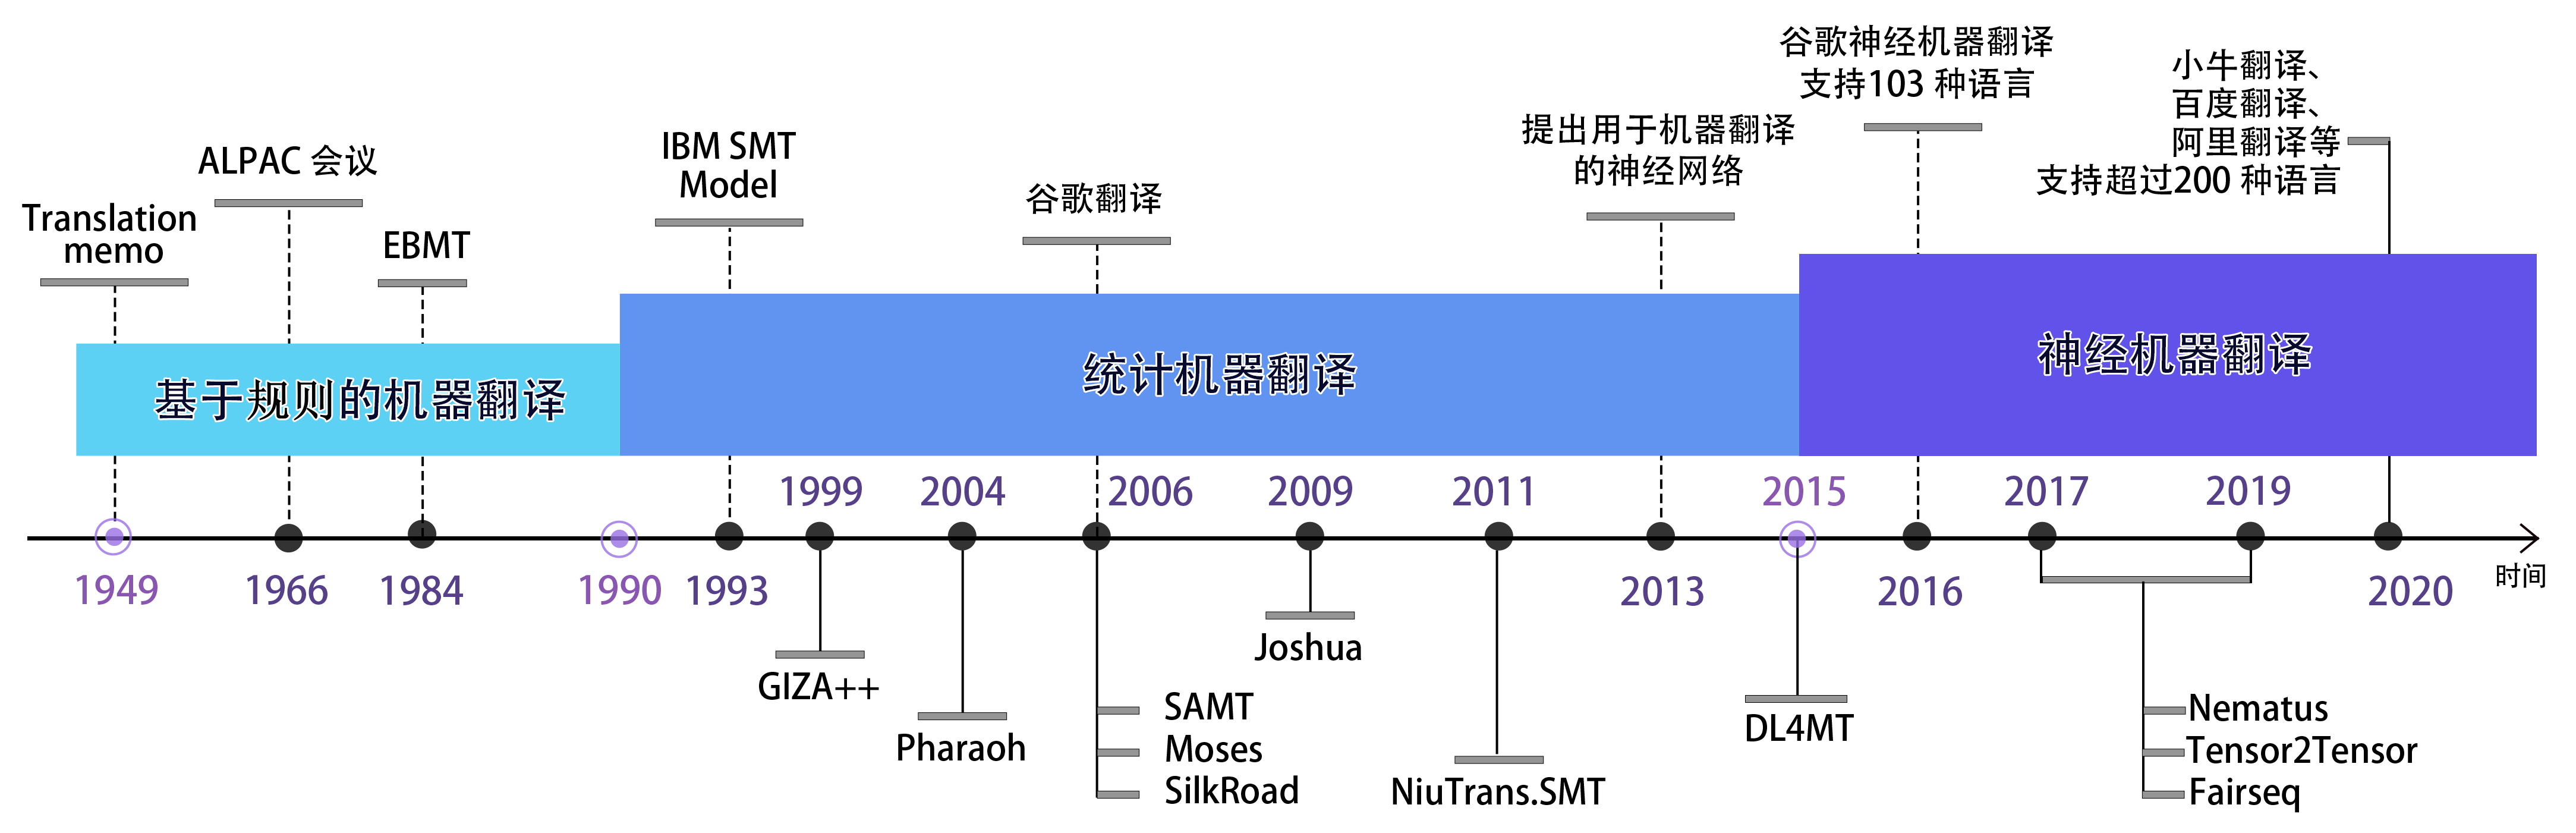
\includegraphics[scale=0.4]{./Chapter10/Figures/mt-history.png}
\caption{机器翻译发展简史}
\label{fig:10-1}
\end{figure}
%----------------------------------------------

\parinterval 神经机器翻译的迅速崛起确实让所有研究人员都有些措手不及,甚至有一种一觉醒来天翻地覆的感觉。也有研究人员评价,神经机器翻译的出现给整个机器翻译领域带来了前所未有的发展机遇。不过,客观地看,机器翻译达到今天这样的状态也是一种历史必然,其中有几方面原因:

\begin{itemize}
\vspace{0.3em}
\item 自上世纪末所发展起来的基于数据驱动的方法为神经机器翻译提供了很好的基础。本质上,神经机器翻译仍然是一种基于统计建模的数据驱动的方法,因此无论是对问题的基本建模方式,还是训练统计模型所使用到的带标注数据,都可以复用机器翻译领域以前的研究成果。特别是机器翻译长期的发展已经积累了大量的双语、单语数据,这些数据在统计机器翻译时代就发挥了很大作用。随着时间的推移,数据规模和质量又得到进一步提升,包括一些评测基准、任务设置都已经非常完备,研究人员可以直接在数据条件全部具备的情况下开展神经机器翻译的研究工作,这些都节省了大量的时间成本。从这个角度说,神经机器翻译是站在巨人的肩膀上才发展起来的。
\vspace{0.3em}
\item 深度学习经过长时间的酝酿终于爆发,为机器翻译等自然语言处理任务提供了新的思路和技术手段。神经机器翻译的不断壮大伴随着深度学习技术的发展。在深度学习的视角下,语言文字可以被表示成抽象的实数向量,这种文字的表示结果可以被自动学习,为机器翻译建模提供了更大的灵活性。相对于神经机器翻译,深度学习的发展更加曲折。虽然深度学习经过了漫长的起伏过程,但是神经机器翻译恰好出现在深度学习逐渐走向成熟的阶段。反过来说,受到深度学习及相关技术空前发展的影响,自然语言处理的范式也发生了变化,神经机器翻译的出现只是这种趋势下的一种必然。
\vspace{0.3em}
\item 此外,计算机算力的提升也为神经机器翻译提供了很好的支撑。与很多神经网络方法一样,神经机器翻译也依赖大量基于浮点数的矩阵运算。甚至在本世纪初,大规模的矩阵运算仍然依赖非常昂贵的CPU集群系统,但是随着GPU等相关技术的发展,在相对低成本的设备上已经可以完成非常复杂的浮点并行运算。这使得包括神经机器翻译在内的很多基于深度学习的系统可以进行大规模实验,随着实验周期的缩短,相关研究和系统的迭代周期也大大缩短。实际上,计算机硬件运算能力一直是稳定提升的,神经机器翻译只是受益于运算能力的阶段性突破。
\vspace{0.3em}
\item 还有,翻译需求的不断增加也为机器翻译技术提供了新的机会。在近几年,无论是翻译品质,还是翻译语种数量,甚至不同的翻译场景,都对机器翻译有了更高的要求。人们迫切需要一种品质更高、翻译效果稳定的机器翻译方法,神经机器翻译恰好满足了这些要求。当然,应用端需求的增加也会反推机器翻译技术的发展,二者相互促进。
\vspace{0.3em}
\end{itemize}

\parinterval 至今,神经机器翻译已经成为带有时代特征的标志性方法。当然,机器翻译的发展也远没有达到终点。下面将介绍神经机器翻译的起源和优势,以便读者在正式了解神经机器翻译的技术方法前对其现状有一个充分的认识。

%----------------------------------------------------------------------------------------
%    NEW SUB-SECTION 10.1.1
%----------------------------------------------------------------------------------------
\subsection{神经机器翻译的起源}
\parinterval 从广义上讲,神经机器翻译是一种基于人工神经网络的方法,它把翻译过程描述为可以用人工神经网络表示的函数,所有的训练和推断都在这些函数上进行。由于神经机器翻译中的神经网络可以用连续可微函数表示,因此这类方法也可以用基于梯度的方法进行优化,相关技术非常成熟。更为重要的是,在神经网络的设计中,研究人员引入了分布式表示的概念,这也是近些年自然语言处理领域的重要成果之一。传统统计机器翻译仍然把词序列看作离散空间里的由多个特征函数描述的点,类似于$n$-gram语言模型,这类模型对数据稀疏问题非常敏感。此外,人工设计特征也在一定程度上限制了模型对问题的表示能力。神经机器翻译把文字序列表示为实数向量,一方面避免了特征工程繁重的工作,另一方面使得系统可以对文字序列的“表示”进行学习。可以说,神经机器翻译的成功很大程度上源自“ 表示学习”这种自然语言处理的新范式的出现。在表示学习的基础上,注意力机制、深度神经网络等技术都被应用于神经机器翻译,使其得以进一步发展。

\parinterval 虽然神经机器翻译中大量地使用了人工神经网络方法,但是它并不是最早在机器翻译中使用人工神经网络的框架。实际上,人工神经网络在机器翻译中应用的历史要远早于现在的神经机器翻译。 在统计机器翻译时代,也有很多研究人员利用人工神经网络进行机器翻译系统模块的构建\upcite{devlin-etal-2014-fast,Schwenk_continuousspace},比如,研究人员成功地在统计机器翻译系统中使用了基于神经网络的联合表示模型,取得了很好的效果\upcite{devlin-etal-2014-fast}。

\parinterval 不过,以上这些工作大多都是在系统的局部模块中使用人工神经网络和深度学习方法。与之不同的是,神经机器翻译是用人工神经网络完成整个翻译过程的建模,这样做的一个好处是,整个系统可以进行端到端学习,无需引入对任何翻译的隐含结构假设。这种利用端到端学习对机器翻译进行神经网络建模的方式也就成为了现在大家所熟知的神经机器翻译。这里简单列出部分代表性的工作:

\begin{itemize}
\vspace{0.3em}
\item 早在2013年,Nal Kalchbrenner和Phil Blunsom提出了一个基于编码器-解码器结构的新模型\upcite{kalchbrenner-blunsom-2013-recurrent}。该模型用卷积神经网络(CNN)将源语言编码成实数向量,之后用循环神经网络(RNN)将连续向量转换成目标语言。这使得模型不需要进行词对齐、特征提取等工作,就能够自动学习源语言的信息。这也是一种端到端学习的方法。不过,这项工作的实现较复杂,而且方法存在梯度消失/爆炸等问题\upcite{HochreiterThe,BENGIO1994Learning},因此并没有成为后来神经机器翻译的基础框架。
\vspace{0.3em}
\item 2014年,Ilya Sutskever等人提出了序列到序列(seq2seq)学习的方法,同时将长短时记忆结构(LSTM)引入到神经机器翻译中,这个方法缓解了梯度消失/爆炸的问题,并且通过遗忘门的设计让网络选择性地记忆信息,缓解了序列中长距离依赖的问题\upcite{NIPS2014_5346}。但是该模型在进行编码的过程中,将不同长度的源语言句子压缩成了一个固定长度的向量,句子越长,损失的信息越多,同时该模型无法对输入和输出序列之间的对齐进行建模,因此并不能有效的保证翻译质量。
\vspace{0.3em}
\item 同年Dzmitry Bahdanau等人首次将{\small\bfnew{注意力机制}}\index{注意力机制}(Attention Mechanism\index{Attention Mechanism})应用到机器翻译领域,在机器翻译任务上对翻译和局部翻译单元之间的对应关系同时建模\upcite{bahdanau2014neural}。Bahdanau等人工作的意义在于,使用了更加有效的模型来表示源语言的信息,同时使用注意力机制对两种语言不同部分之间的相互联系进行建模。这种方法可以有效地处理长句子的翻译,而且注意力的中间结果具有一定的可解释性\footnote{比如,目标语言和源语言句子不同单词之间的注意力强度能够在一定程度上反应单词之间的互译程度。} 。然而相比于前人的神经机器翻译模型,注意力模型也引入了额外的成本,计算量较大。
\vspace{0.3em}
\item 2016年谷歌公司发布了基于多层循环神经网络方法的GNMT系统。该系统集成了当时的神经机器翻译技术,并进行了诸多的改进。它的性能显著优于基于短语的机器翻译系统\upcite{Wu2016GooglesNM},引起了研究人员的广泛关注。在之后不到一年的时间里,脸书公司采用卷积神经网络(CNN)研发了新的神经机器翻译系统\upcite{DBLP:journals/corr/GehringAGYD17},实现了比基于循环神经网络(RNN)系统更高的翻译水平,并大幅提升翻译速度。
\vspace{0.3em}
\item 2017年,Ashish Vaswani等人提出了新的翻译模型Transformer。其完全摒弃了循环神经网络和卷积神经网络,仅仅通过多头注意力机制和前馈神经网络,不需要使用序列对齐的循环框架就展示出强大的性能,并且巧妙地解决了翻译中长距离依赖问题\upcite{vaswani2017attention}。Transformer是第一个完全基于注意力机制搭建的模型,不仅训练速度更快,在翻译任务上也获得了更好的结果,一跃成为目前最主流的神经机器翻译框架。
\vspace{0.3em}
\end{itemize}

\parinterval  当然,神经机器翻译的工作远不止以上这些内容\upcite{StahlbergNeural}。随着本书内容的逐渐深入,很多经典的模型和方法都会被讨论到。

%----------------------------------------------------------------------------------------
%    NEW SUB-SECTION 10.1.2
%----------------------------------------------------------------------------------------
\subsection{神经机器翻译的品质}
\parinterval  图\ref{fig:10-2}展示了用机器翻译把一段汉语翻译为英语的结果。其中译文1是统计机器翻译系统的结果,译文2是神经机器翻译系统的结果。为了保证公平性,两个系统使用完全相同的数据进行训练。

%----------------------------------------------
%\begin{figure}[htp]
%\centering
%\input{./Chapter10/Figures/figure-example-of-mt-1}
%\setlength{\abovecaptionskip}{-0.2cm}
%\caption{机器翻译实例对比}
%\label{fig:10-2}
%\end{figure}
%----------------------------------------------

%----------------------------------------------
\begin{figure}[htp]
\centering
\input{./Chapter10/Figures/figure-example-of-mt}
%\setlength{\abovecaptionskip}{-0.2em}
\caption{机器翻译实例对比}
\label{fig:10-2}
\end{figure}
%----------------------------------------------

\vspace{-0.3em}
\parinterval  可以明显地看到译文2更加通顺,意思的表达更加准确,翻译质量明显高于译文1。这个例子基本反应出统计机器翻译和神经机器翻译的差异性。当然,这里并不是要讨论统计机器翻译和神经机器翻译孰优孰劣,只是很多场景中发现神经机器翻译系统可以生成非常流畅的译文,易于人工阅读和修改。

\parinterval  在很多量化的评价中也可以看到神经机器翻译的优势。回忆一下{\chapterfour}提到的机器翻译质量的自动评估指标中,使用最广泛的一种指标是BLEU。2010年前,在由美国国家标准和科技机构(NIST)举办的汉英机器翻译评测中(比如汉英MT08数据集),30\%以上的BLEU值对于基于统计方法的翻译系统来说就已经是当时最顶尖的结果了。而现在的神经机器翻译系统,则可以轻松地将BLEU提高至45\%以上。

\parinterval  同样,在机器翻译领域中著名评测比赛WMT(Workshop of Machine Translation)中,使用统计机器翻译方法的参赛系统也在逐年减少。而现在获得比赛冠军的系统中几乎没有只使用纯统计机器翻译模型的系统\footnote{但是,仍然有大量的统计机器翻译和神经机器翻译融合的方法。比如,在无指导机器翻译中,统计机器翻译仍然被作为初始模型。} 。图\ref{fig:10-3}展示了近年来WMT比赛冠军系统中神经机器翻译系统的数量,可见神经机器翻译系统的数量在逐年提高。

%----------------------------------------------
\begin{figure}[htp]
\centering
\input{./Chapter10/Figures/figure-numbers-of-wmt-systems}
\caption{WMT冠军系统的数量}
\label{fig:10-3}
\end{figure}
%----------------------------------------------

\parinterval  神经机器翻译在其他评价指标上的表现也全面超越统计机器翻译。比如,在IWSLT 2015英语-德语任务中,研究人员搭建了四个较为先进的机器翻译系统\upcite{Bentivogli2016NeuralVP}:

\begin{itemize}
\vspace{0.3em}
\item PBSY:基于短语和串到树模型的混合系统,其中也使用了一些稀疏的词汇化特征;
\vspace{0.3em}
\item HPB:层次短语系统,其中使用了基于句法的预调序和基于神经语言模型的重排序模块;
\vspace{0.3em}
\item SPB:标准的基于短语的模型,其中使用了基于神经语言模型的重排序模块;
\vspace{0.3em}
\item NMT:神经机器翻译系统,其中使用了长短时记忆模型、注意力机制、稀有词处理机制等。
\end{itemize}

\parinterval  与这些系统相比,神经机器翻译系统的mTER得分在不同长度句子上都有明显的下降,如图\ref{fig:10-4}\footnote{mTER、HTER等都是是错误率度量,值越低表明译文越好。}。其次,神经机器翻译的单词形态错误率和单词词义错误率(用HTER度量)都远低于统计机器翻译系统(表\ref{tab:10-1} )。

%----------------------------------------------
\begin{figure}[htp]
\centering
\input{./Chapter10/Figures/figure-score-of-mter}
\caption{不同系统在不同长度句子上的mTER[\%]分值(得分越低越好)\upcite{Bentivogli2016NeuralVP}}
\label{fig:10-4}
\end{figure}
%----------------------------------------------

\vspace{0.5em}%全局布局使用
%----------------------------------------------
\begin{table}[htp]
\centering
\caption{神经机器翻译与统计机器翻译系统的译文错误率HTER[\%](忽略编辑距离中的移动操作)\upcite{Bentivogli2016NeuralVP}}
\label{tab:10-1}
\begin{tabular}{r|llc}
系统                    & 单词 & 词根 & Δ \\ \hline
PBSY                    & 27.1          & 22.5           & -16.9       \\
HPB                     & 28.7          & 23.5           & -18.4       \\
SPB                     & 28.3          & 23.2           & -18.0       \\
NMT                     & 21.7          & 18.7           & -13.7      \\
\end{tabular}
\end{table}
%----------------------------------------------

\parinterval 此外,神经机器翻译在某些任务上的结果已经相当优秀,比如,在一些汉英新闻翻译任务中,神经机器翻译就取得了至少和专业翻译人员相媲美的效果\upcite{Hassan2018AchievingHP}。在该任务中,神经机器系统(Combo-4、Combo-5 和 Combo-6)的人工评价得分与Reference-HT(专业翻译人员翻译)的得分无显著差别,且远超Reference-WMT(WMT的参考译文,也是由人类翻译)得分(表\ref{tab:10-2})。

\vspace{0.5em}%全局布局使用
%----------------------------------------------
\begin{table}[htp]
\centering
\caption{不同机器翻译系统人类评价结果\upcite{Hassan2018AchievingHP}}
\label{tab:10-2}
\begin{tabular}{l | l l}
	\# 		&\begin{tabular}[c]{@{}l@{}}Ave\%\\ (平均原始分数)\end{tabular}		&系统 \\ \hline
	1 		&69.0			&Combo-6 \\
			&68.5			&Reference-HT \\
			&68.9			&Combo-5 \\
			&68.6			&Combo-4 \\
	2		&62.1			&Reference-WMT \\
\end{tabular}
\end{table}
%----------------------------------------------

\parinterval  在最近两年,神经机器翻译的发展更加迅速,新的模型及方法层出不穷。表\ref{tab:10-3}给出了到2020年为止,一些主流的神经机器翻译模型在WMT14英德数据集上的表现。可以看到,相比2017年,2018-2020年中机器翻译仍然有进步。

\vspace{0.5em}%全局布局使用
%----------------------------------------------
\begin{table}[htp]
\centering
\caption{WMT14英德数据集上不同神经机器翻译模型的表现}
\label{tab:10-3}
\begin{tabular}{ l | l l l}
   模型         		 &作者	& 年份	& BLEU[\%] \\ \hline
   \rule{0pt}{13pt}ConvS2S \upcite{DBLP:journals/corr/GehringAGYD17}                			&Gehring等 		&2017 			&25.2 \\
   Transformer-Base \upcite{vaswani2017attention}			&Vaswani等 		&2017 			&27.3 \\
   Transformer-Big  \upcite{vaswani2017attention} 			&Vaswani等 		&2017 			&28.4 \\
   RNMT+		 \upcite{Chen2018TheBO}			&Chen等 	  	&2018  			&28.5 \\
   Layer-Wise Coordination \upcite{He2018LayerWiseCB}	&He等 	 		&2018 			&29.0 \\
   Transformer-RPR	\upcite{Shaw2018SelfAttentionWR}	 	&Shaw等 	 	&2018 			&29.2 \\
   Transformer-DLCL	\upcite{WangLearning}		 &Wang等 	 	&2019 			&29.3 \\
   SDT                \upcite{li2020shallow}                 &Li等 &2020 & 30.4 \\
   MSC                  \upcite{Wei2020MultiscaleCD}    &Wei等   &2020  &30.5 \\
\end{tabular}
\end{table}
%----------------------------------------------

%----------------------------------------------------------------------------------------
%    NEW SUB-SECTION 10.1.3
%----------------------------------------------------------------------------------------
\subsection{神经机器翻译的优势}

\parinterval  既然神经机器翻译如此强大,它的优势在哪里呢?为了回答这个问题,表\ref{tab:10-4}给出了神经机器翻译与统计机器翻译的简单对比。具体来说,神经机器翻译有如下特点:

%----------------------------------------------
\begin{table}[htp]
\centering
\caption{统计机器翻译 vs 神经机器翻译}
\label{tab:10-4}
\begin{tabular}{ l | l }
  \rule{0pt}{15pt}  \parbox{12em}{统计机器翻译		}	&神经机器翻译\\ \hline
	  \rule{0pt}{13pt}  基于离散空间的表示模型			&基于连续空间的表示模型 \\
	  \rule{0pt}{13pt} NLP问题的隐含结构假设			&无隐含结构假设,端到端学习 \\
	  \rule{0pt}{13pt} 特征工程为主					&不需要特征工程,但需要设计网络 \\
	  \rule{0pt}{13pt} 特征、规则的存储耗资源			&模型存储相对小,但计算量大 \\
\end{tabular}
\end{table}
%----------------------------------------------


\begin{itemize}
\vspace{0.5em}
\item 连续空间表示模型,能捕获更多隐藏信息。神经机器翻译与统计机器翻译最大的区别在于对语言文字串的表示方法。在统计机器翻译中,所有词串本质上都是由更小的词串(短语、规则)组合而成,也就是统计机器翻译模型利用了词串之间的组合性来表示更大的词串。统计机器翻译使用多个特征描述翻译结果,但是其仍然对应着离散的字符串的组合,因此可以把模型对问题的表示空间看做是由一个离散结构组成的集合。在神经机器翻译中,词串的表示已经被神经网络转化为多维实数向量,而且也不依赖任何的可组合性假设等其他假设来刻画离散的语言结构,从这个角度说,所有的词串分别对应了一个连续空间上的点(比如,对应多维实数空间中一个点)。这样,模型可以更好地进行优化,而且对未见样本有更好的泛化能力。此外,基于连续可微函数的机器学习算法已经相对完备,可以很容易地对问题进行建模和优化。

\vspace{0.5em}
\item 不含隐含结构假设,端到端学习对问题建模更加直接。传统的自然语言处理任务会对问题进行隐含结构假设。比如,进行翻译时,统计机器翻译会假设翻译过程由短语的拼装完成。这些假设可以大大化简问题的复杂度,但是另一方面也带来了各种各样的约束条件,并且错误的隐含假设往往会导致建模错误。神经机器翻译是一种端到端模型,它并不依赖任何隐含结构假设。这样,模型并不会受到错误的隐含结构的引导。从某种意义上说,端到端学习可以让模型更加“ 自由”地进行学习,因此往往可以学到很多传统认知上不容易理解或者不容易观测到的现象。

\vspace{0.5em}
\item 不需要特征工程,特征学习更加全面。经典的统计机器翻译可以通过判别式模型引入任意特征,不过这些特征需要人工设计,因此这个过程也被称为特征工程。特征工程依赖大量的人工,特别是对不同语种、不同场景的翻译任务,所采用的特征可能不尽相同,这也使得设计有效的特征成为了统计机器翻译时代最主要的工作之一。但是,由于人类自身的思维和认知水平的限制,人工设计的特征可能不全面,甚至会遗漏一些重要的翻译现象。神经机器翻译并不依赖任何人工特征的设计,或者说它的特征都隐含在分布式表示中。这些“特征”都是自动学习得到的,因此神经机器翻译并不会受到人工思维的限制,学习到的特征将问题描述得更全面。

\vspace{0.5em}
\item 模型结构统一,存储相对更小。统计机器翻译系统依赖于很多模块,比如词对齐、短语(规则)表和目标语言模型等等,因为所有的信息(如$n$-gram)都是离散化表示的,因此模型需要消耗大量的存储资源。同时,由于系统模块较多,开发的难度也较大。神经机器翻译的模型都是用神经网络进行表示,模型参数大多是实数矩阵,因此存储资源的消耗很小。而且神经网络可以作为一个整体进行开发和调试,系统搭建的代价相对较低。实际上,由于模型体积小,神经机器翻译也非常合适于离线小设备上的翻译任务。

\vspace{0.5em}
\end{itemize}

\parinterval  当然,神经机器翻译也并不完美,很多问题有待解决。首先,神经机器翻译需要大规模浮点运算的支持,模型的推断速度较低。为了获得优质的翻译结果,往往需要大量GPU设备的支持,计算资源成本很高;其次,由于缺乏人类的先验知识对翻译过程的指导,神经机器翻译的运行过程缺乏可解释性,系统的可干预性也较差;此外,虽然脱离了繁重的特征工程,神经机器翻译仍然需要人工设计网络结构,在模型的各种超参数的设置、训练策略的选择等方面,仍然需要大量的人工参与。这也导致很多实验结果不容易复现。显然,完全不依赖人工的机器翻译还很遥远。不过,随着研究人员的不断攻关,很多问题也得到了解决。

%----------------------------------------------------------------------------------------
%    NEW SECTION  10.2
%----------------------------------------------------------------------------------------
\sectionnewpage
\section{编码器-解码器框架}

\parinterval 说到神经机器翻译就不得不提{\small\bfnew{编码器-解码器模型}}\index{编码器-解码器模型},或{\small\bfnew{编码器-解码器框架}} \index{编码器-解码器框架}(Encoder-Decoder Paradigm)\index{Encoder-Decoder Paradigm}。本质上,编码器-解码器模型是描述输入-输出之间关系的一种方式。编码器-解码器这个概念在日常生活中并不少见。例如,在电视系统上为了便于视频的传播,会使用各种编码器将视频编码成数字信号,在客户端,相应的解码器组件会把收到的数字信号解码为视频。另外一个更贴近生活的例子是电话,它通过对声波和电信号进行相互转换,达到传递声音的目的。这种“先编码,再解码”的思想被应用到密码学、信息论等多个领域。

\parinterval 不难看出,机器翻译问题也完美的贴合编码器-解码器结构的特点。可以将源语言编码为类似信息传输中的数字信号,然后利用解码器对其进行转换,生成目标语言。下面就来看一下神经机器翻译是如何在编码器-解码器框架下进行工作的。

%----------------------------------------------------------------------------------------
%    NEW SUB-SECTION 10.2.1
%----------------------------------------------------------------------------------------
\subsection{框架结构}

\parinterval  编码器-解码器框架是一种典型的基于“表示”的模型。编码器的作用是将输入的文字序列通过某种转换变为一种新的“表示”形式,这种“表示”包含了输入序列的所有信息。之后,解码器把这种“表示”重新转换为输出的文字序列。这其中的一个核心问题是表示学习,即:如何定义对输入文字序列的表示形式,并自动学习这种表示,同时应用它生成输出序列。一般来说,不同的表示学习方法可以对应不同的机器翻译模型,比如,在最初的神经机器翻译模型中,源语言句子都被表示为一个独立的向量,这时表示结果是静态的;而在注意力机制中,源语言句子的表示是动态的,也就是翻译目标语言的每个单词时都会使用不同的表示结果。

\parinterval  图\ref{fig:10-5}是一个应用编码器-解码器结构来解决机器翻译问题的简单实例。给定一个中文句子“我/对/你/感到/满意”,编码器会将这句话编码成一个实数向量$(0.2, -1, 6, \\ 5, 0.7, -2)$,这个向量就是源语言句子的“表示”结果。虽然有些不可思议,但是神经机器翻译模型把这个向量等同于输入序列。向量中的数字并没有实际的意义,然而解码器却能从中提取到源语言句子中所包含的信息。也有研究人员把向量的每一个维度看作是一个“特征”,这样源语言句子就被表示成多个“特征”的联合,而且这些特征可以被自动学习。有了这样的源语言句子的“表示”,解码器可以把这个实数向量作为输入,然后逐词生成目标语言句子“I am satisfied with you”。

%----------------------------------------------
\begin{figure}[htp]
\centering
\input{./Chapter10/Figures/figure-encoder-decoder-process}
\caption{使用编码器-解码器架构处理汉英翻译的过程 }
\label{fig:10-5}
\end{figure}
%----------------------------------------------

\parinterval  在源语言句子的表示形式确定之后,需要设计相应的编码器和解码器结构。在当今主流的神经机器翻译系统中,编码器由词嵌入层和中间网络层组成。当输入一串单词序列时,词嵌入层会将每个单词映射到多维实数表示空间,这个过程也被称为词嵌入。之后中间层会对词嵌入向量进行更深层的抽象,得到输入单词序列的中间表示。中间层的实现方式有很多,比如:循环神经网络、卷积神经网络、自注意力机制等都是模型常用的结构。解码器的结构基本上和编码器是一致的,在基于循环神经网络的翻译模型中,解码器只比编码器多了输出层,用于输出每个目标语言位置的单词生成概率,而在基于自注意力机制的翻译模型中,除了输出层,解码器还比编码器多一个编码-解码注意力子层,用于帮助模型更好地利用源语言信息。

\parinterval  现在,编码器-解码器框架已经成为了神经机器翻译系统的标准架构。当然,也有一些研究工作在探索编码器-解码器框架之外的结构\upcite{Li2020NeuralMT},但是还没有太多颠覆性的进展。因此,本章仍然以编码器-解码器框架为基础对相关模型和方法进行介绍。

%----------------------------------------------------------------------------------------
%    NEW SUB-SECTION 10.2.2
%----------------------------------------------------------------------------------------
\subsection{表示学习}

\parinterval 编码器-解码器框架的创新之处在于,将传统基于符号的离散型知识转化为分布式的连续型知识。比如,对于一个句子,它可以由离散的符号所构成的文法规则来生成,也可以直接被表示为一个实数向量记录句子的各个“属性”。这种分布式的实数向量可以不依赖任何离散化的符号系统,简单来说,它就是一个函数,把输入的词串转化为实数向量。更为重要的是,这种分布式表示可以被自动学习。或者从某种意义上说,编码器-解码器框架的作用之一就是学习输入序列的表示。表示结果学习的好与坏很大程度上会影响神经机器翻译系统的性能。

\parinterval 图\ref{fig:10-6}对比了统计机器翻译和神经机器翻译的表示模型的区别。传统的统计机器翻译(a)通过短语或者规则组合来获得更大的翻译片段,直至覆盖整个句子。这本质上是在一个离散的结构空间中不断组合的过程。神经机器翻译(b)与之不同,它并没有所谓的“组合”的过程,整个句子的处理是直接在连续空间上进行计算得到的。这二者的区别也体现了符号系统与神经网络系统的区别。前者更适合处理离散化的结构表示,后者更适合处理连续化的表示。

%----------------------------------------------
\begin{figure}[htp]
    \centering
    \input{./Chapter10/Figures/figure-presentation-space}
    \caption{统计机器翻译和神经机器翻译的表示空间}
    \label{fig:10-6}
\end{figure}
%----------------------------------------------

\parinterval 实际上,编码器-解码器模型也并不是表示学习实现的唯一途径。比如,在{\chapternine}提到的神经语言模型实际上也是一种有效的学习句子表示的方法,它所衍生出的预训练模型可以从大规模单语数据上学习句子的表示形式。这种学习会比使用少量的双语数据进行编码器和解码器的学习更加充分。相比机器翻译任务,语言模型相当于一个编码器的学习 \footnote{相比神经机器翻译的编码器,神经语言模型会多出一个输出层,这时可以直接把神经语言模型的中间层的输出作为编码器的输出。},可以无缝嵌入到神经机器翻译模型中。不过,值得注意的是,机器翻译的目的是解决双语字符串之间的映射问题,因此它所使用的句子表示是为了更好地进行翻译。从这个角度说,机器翻译中的表示学习又和语言模型中的表示学习有不同。不过,这里不会深入讨论神经语言模型和预训练与神经机器翻译之间的异同,在后续章节会有相关讨论。

\parinterval 还有一点,在神经机器翻译中,句子的表示形式可以有很多选择。使用单个向量表示一个句子是一种最简单的方法。当然,也可以用矩阵、高阶张量完成表示。甚至,在解码时动态地生成源语言的表示结果。

%----------------------------------------------------------------------------------------
%    NEW SUB-SECTION 10.2.3
%----------------------------------------------------------------------------------------
\subsection{简单的运行实例}

\parinterval 为了对编码器-解码器框架和神经机器翻译的运行过程有一个直观的认识,这里采用标准的循环神经网络作为编码器和解码器的结构,演示一个简单的翻译实例。假设系统的输入和输出为:

\vspace{0.5em}
\parinterval  \hspace{5em} 输入(汉语):我\ \ 很\ \  好\ \ <eos>

\vspace{0.3em}
\parinterval  \hspace{5em} 输出(英语):I\ \ am\ \ fine\ \ <eos>
\vspace{0.5em}

\noindent 这里令<eos>(End of Sequence)表示序列的终止,<sos>(Start of Sequence)表示序列的开始。

%----------------------------------------------
\begin{figure}[htp]
\centering
\input{./Chapter10/Figures/figure-a-working-example-of-neural-machine-translation}
\caption{神经机器翻译的运行实例}
\label{fig:10-7}
\end{figure}
%----------------------------------------------

\parinterval 翻译过程的神经网络结构如图\ref{fig:10-7}所示,其中左边是编码器,右边是解码器。编码器会顺序处理源语言单词,将每个单词都表示成一个实数向量,也就是每个单词的词嵌入结果(绿色方框)。在词嵌入的基础上运行循环神经网络(蓝色方框)。在编码下一个时间步状态的时候,上一个时间步的隐藏状态会作为历史信息传入循环神经网络。这样,句子中每个位置的信息都被向后传递,最后一个时间步的隐藏状态(红色方框)就包含了整个源语言句子的信息,也就得到了编码器的编码结果$\ \dash\ $源语言句子的分布式表示。

\parinterval 解码器直接把源语言句子的分布式表示作为输入的隐藏层状态,之后像编码器一样依次读入目标语言单词,这是一个标准的循环神经网络的执行过程。与编码器不同的是,解码器会有一个输出层,用于根据当前时间步的隐藏层状态生成目标语言单词及其概率分布。可以看到,解码器当前时刻的输出单词与下一个时刻的输入单词是一样的。从这个角度说,解码器也是一种神经语言模型,只不过它会从另外一种语言(源语言)获得一些信息,而不是仅仅生成单语句子。具体来说,当生成第一个单词“I”时,解码器利用了源语言句子表示(红色方框)和目标语言的起始词“<sos>”。在生成第二个单词“am”时,解码器利用了上一个时间步的隐藏状态和已经生成的“I”的信息。这个过程会循环执行,直到生成完整的目标语言句子。

\parinterval 从这个例子可以看出,神经机器翻译的流程其实并不复杂:首先通过编码器神经网络将源语言句子编码成实数向量,然后解码器神经网络利用这个向量逐词生成译文。现在几乎所有的神经机器翻译系统都采用类似的架构。

%----------------------------------------------------------------------------------------
%    NEW SUB-SECTION 10.2.4
%----------------------------------------------------------------------------------------
\subsection{机器翻译范式的对比}

\parinterval 对于不同类型的机器翻译方法,人类所扮演的作用是不同的。在统计机器翻译时代,往往需要人工定义所需要的特征和翻译单元,翻译中的每一个步骤对于人来说都是透明的,翻译过程具有一定的可解释性。而在神经机器翻译时代,神经机器翻译将所有的工作都交给神经网络,翻译的过程完全由神经网络计算得到。在整个神经网络的运行过程中并不需要人工先验知识,其中所生成的中间表示也只有神经网络自身才可以理解。有时候也会把神经机器翻译系统看作“黑盒”。所谓“黑盒”并不是指神经网络计算的过程不可见,而是这种复杂的计算过程无法控制也很难解释。那么是神经机器翻译会魔法吗,不需要任何人为的干预就可以进行翻译吗?其实不然,相对于统计机器翻译,真正变化的是人类使用知识的形式。

\parinterval 在机器翻译的不同时期,人类参与到机器翻译中的形式并不相同,如表\ref{tab:10-5}所述。具体来说,

\begin{itemize}
\item 在早期基于规则的方法中,规则的编写、维护均需要人来完成,也就是人类直接提供了计算机可读的知识形式;
\item 在统计机器翻译方法中,则需要人为的设计翻译特征,并且定义基本翻译单元的形式,然后剩下的事情(比如翻译过程)交由统计机器翻译算法完成,也就是人类间接的提供了翻译所需要的知识;
\item 在神经机器翻译方法中,特征的设计完全不需要人的参与,但是进行特征提取的网络结构仍然需要人为地设计,训练网络所需要的参数也需要工程师的不断调整,才能发挥神经机器翻译的强大性能。
\end{itemize}

%----------------------------------------------
\begin{table}[htp]
\centering
\caption{不同机器翻译范式中人类的作用}
\label{tab:10-5}
\begin{tabular}{ l | l }
	机器翻译方法			&人类参与方式 \\ \hline
	\rule{0pt}{13pt} 基于规则的方法					&设计翻译规则 \\
	\rule{0pt}{13pt} 传统统计方法					&设计翻译特征 \\
	\rule{0pt}{13pt} 神经网络方法					&设计网络架构 \\
\end{tabular}
\end{table}
%----------------------------------------------

\parinterval 可见,不管是基于规则的机器翻译方法,还是统计机器翻译方法,甚至最新的神经机器翻译方法,人类的作用是不可替代的。虽然神经机器翻译很强大,但是它的成功仍然依赖人工设计网络结构、调参。纵然,也有一些研究工作通过结构搜索的方法自动获得神经网络结构,但是搜索的算法和模型仍然需要人工设计。道理很简单:机器翻译是人类设计的,脱离了人的工作,机器翻译是不可能成功的。

%----------------------------------------------------------------------------------------
%    NEW SECTION   10.3
%----------------------------------------------------------------------------------------
\sectionnewpage
\vspace{-2em}
\section{基于循环神经网络的翻译建模}

\parinterval 早期神经机器翻译的进展主要来自两个方面:1)使用循环神经网络对单词序列进行建模;2)注意力机制的使用。表\ref{tab:10-6}列出了2013-2015年间有代表性的部分研究工作。从这些工作的内容上看,当时的研究重点还是如何有效地使用循环神经网络进行翻译建模以及使用注意力机制捕捉双语单词序列间的对应关系。

%----------------------------------------------
\begin{table}[htp]
\centering
\caption{2013-2015期间神经机器翻译方面的部分论文}
\label{tab:10-6}
\begin{tabular}{l| l p{8cm}}
\rule{0pt}{16pt} 时间   & 作者                                                              & 论文                                                                      \\ \hline
\rule{0pt}{0pt} 2013 & \begin{tabular}[c]{@{}l@{}l@{}}\\Kalchbrenner\\ 和Blunsom\end{tabular} & Recurrent Continuous Translation Models \upcite{kalchbrenner-blunsom-2013-recurrent}                                \\
\rule{0pt}{16pt} 2014 & Sutskever等                                                       & Sequence to Sequence Learning with neural networks \upcite{NIPS2014_5346}                     \\
\rule{0pt}{16pt} 2014 & Bahdanau等                                                       & Neural Machine Translation by Jointly Learning to Align and Translate \upcite{bahdanau2014neural} \\
\rule{0pt}{16pt} 2014 & Cho等                                                            & On the Properties of Neural Machine Translation \upcite{cho-etal-2014-properties}                        \\
\rule{0pt}{16pt} 2015 & Jean等                                                           & On Using Very Large Target Vocabulary for Neural Machine Translation \upcite{DBLP:conf/acl/JeanCMB15}   \\
\rule{0pt}{16pt} 2015 & Luong等                                                          & Effective Approches to Attention-based Neural Machine Translation \upcite{DBLP:journals/corr/LuongPM15}
\end{tabular}
\end{table}
%----------------------------------------------

\parinterval 可以说循环神经网络和注意力机制构成了当时神经机器翻译的标准框架。例如,2016年出现的GNMT(Google's Neural Machine Translation)系统就是由多层循环神经网络(长短时记忆模型)以及注意力机制搭建,且在当时展示出很出色的性能\upcite{Wu2016GooglesNM}。其中的很多技术也都为其它神经机器翻译系统的研发提供了很好的依据。

\parinterval 下面将会从基于循环神经网络的翻译模型入手,介绍神经机器翻译的基本方法。之后,会对注意力机制进行介绍,同时也会介绍其在GNMT系统中的应用。

%----------------------------------------------------------------------------------------
%    NEW SUB-SECTION
%----------------------------------------------------------------------------------------
\subsection{建模}
\label{sec:10.3.1}

\parinterval 同大多数自然语言处理任务一样,神经机器翻译要解决的一个基本问题是如何描述文字序列,称为序列表示问题。例如,语音数据、文本数据的处理问题都可以被看作经典的序列表示问题。如果把一个序列看作一个时序上的一系列变量,不同时刻的变量之间往往是存在相关性的。也就是说,一个时序中某个时刻变量的状态会依赖其他时刻变量的状态,即上下文的语境信息。下面是一个简单的例子,假设有一个句子,但是最后的单词被擦掉了,如何猜测被擦掉的单词是什么?

\vspace{0.8em}
\centerline{中午\ 没\ 吃饭\ ,\ 又\ 刚\ 打\ 了\ 一\ 下午\ 篮球\ ,\ 我\ 现在\ 很\ 饿\ ,\ 我\ 想\underline{\quad \quad \quad} 。}
\vspace{0.8em}

\parinterval 显然,根据上下文中提到的“没/吃饭”、“很/饿”,最佳的答案是“吃饭”或者“吃东西”。也就是,对序列中某个位置的答案进行预测时需要记忆当前时刻之前的序列信息,因此,循环神经网络应运而生。实际上循环神经网络有着极为广泛的应用,例如语音识别、语言建模以及即将要介绍的神经机器翻译。

\parinterval {\chapternine}已经对循环神经网络的基本知识进行过介绍,这里再回顾一下。简单来说,循环神经网络由循环单元组成。对于序列中的任意时刻,都有一个循环单元与之对应,它会融合当前时刻的输入和上一时刻循环单元的输出,生成当前时刻的输出。这样每个时刻的信息都会被传递到下一时刻,这也间接达到了记录历史信息的目的。比如,对于序列$\seq{x}=\{x_1,..., x_m\}$,循环神经网络会按顺序输出一个序列$\seq{h}=\{ \mathbi{h}_1,..., \mathbi{h}_m \}$,其中$\mathbi{h}_i$表示$i$时刻循环神经网络的输出(通常为一个向量)。

\parinterval 图\ref{fig:10-8}展示了一个循环神经网络处理序列问题的实例。当前时刻循环单元的输入由上一个时刻的输出和当前时刻的输入组成,因此也可以理解为,网络当前时刻计算得到的输出是由之前的序列共同决定的,即网络在不断地传递信息的过程中记忆了历史信息。以最后一个时刻的循环单元为例,它在对“开始”这个单词的信息进行处理时,参考了之前所有词(“<sos>\ 让\ 我们”)的信息。

%----------------------------------------------
\begin{figure}[htp]
\centering
\input{./Chapter10/Figures/figure-structure-of-a-recurrent-network-model}
\caption{循环神经网络处理序列的实例}
\label{fig:10-8}
\end{figure}
%----------------------------------------------

\parinterval 在神经机器翻译里使用循环神经网络也很简单。只需要把源语言句子和目标语言句子分别看作两个序列,之后使用两个循环神经网络分别对其进行建模。这个过程如图\ref{fig:10-9}所示。图中,下半部分是编码器,上半部分是解码器。编码器利用循环神经网络对源语言序列逐词进行编码处理,同时利用循环单元的记忆能力,不断累积序列信息,遇到终止符<eos>后便得到了包含源语言句子全部信息的表示结果。解码器利用编码器的输出和起始符<sos>开始逐词地进行解码,即逐词翻译,每得到一个译文单词,便将其作为当前时刻解码器端循环单元的输入,这也是一个典型的神经语言模型的序列生成过程。解码器通过循环神经网络不断地累积已经得到的译文的信息,并继续生成下一个单词,直到遇到结束符<eos>,便得到了最终完整的译文。

%----------------------------------------------
\begin{figure}[htp]
\centering
\input{./Chapter10/Figures/figure-model-structure-based-on-recurrent-neural-network-translation}
\caption{基于循环神经网络翻译的模型结构}
\label{fig:10-9}
\end{figure}
%----------------------------------------------

\parinterval 从数学模型上看,神经机器翻译模型与统计机器翻译模型的目标是一样的:在给定源语言句子$\seq{x}$的情况下,找出翻译概率最大的目标语言译文$\hat{\seq{y}}$,其计算如下式:
\vspace{-1em}
\begin{eqnarray}
\hat{\seq{{y}}} &=& \argmax_{\seq{{y}}} \funp{P} (\seq{{y}} | \seq{{x}})
\label{eq:10-1}
\end{eqnarray}

\noindent 这里,用$\seq{{x}}=\{ x_1,..., x_m \}$表示输入的源语言单词序列,$\seq{{y}}=\{ y_1,..., y_n \}$ 表示生成的目标语言单词序列。由于神经机器翻译在生成译文时采用的是自左向右逐词生成的方式,并在翻译每个单词时考虑已经生成的翻译结果,因此对$ \funp{P} (\seq{{y}} | \seq{{x}})$的求解可以转换为下式:
\begin{eqnarray}
\funp{P} (\seq{{y}} | \seq{{x}}) &=& \prod_{j=1}^{n} \funp{P} ( y_j | \seq{{y}}_{<j }, \seq{{x}}  )
\label{eq:10-2}
\end{eqnarray}

\vspace{-0.5em}
\noindent 其中,$ \seq{{y}}_{<j }$表示目标语言第$j$个位置之前已经生成的译文单词序列。$ \funp{P} ( y_j | \seq{{y}}_{<j }, \seq{{x}})$可以被解释为:根据源语言句子$\seq{{x}} $和已生成的目标语言译文片段$\seq{{y}}_{<j }=\{ y_1,..., y_{j-1} \}$,生成第$j$个目标语言单词$y_j$的概率。

\parinterval 求解$\funp{P}(y_j | \seq{{y}}_{<j},\seq{{x}})$有三个关键问题(图\ref{fig:10-10}):

\vspace{-0.5em}
\begin{itemize}
\vspace{0.5em}
\item	如何对$\seq{{x}}$和$\seq{{y}}_{<j }$进行分布式表示,即词嵌入。首先,将由One-hot向量表示的源语言单词,即由0和1构成的离散化向量表示,转化为实数向量。可以把这个过程记为$\textrm{e}_x (\cdot)$。类似地,可以把目标语言序列$\seq{{y}}_{<j }$中的每个单词用同样的方式进行表示,记为$\textrm{e}_y (\cdot)$。
\vspace{0.5em}
\item	如何在词嵌入的基础上获取整个序列的表示,即句子的表示学习。可以把词嵌入的序列作为循环神经网络的输入,循环神经网络最后一个时刻的输出向量便是整个句子的表示结果。如图\ref{fig:10-10}中,编码器最后一个循环单元的输出$\mathbi{h}_m$被看作是一种包含了源语言句子信息的表示结果,记为$\mathbi{C}$。
\vspace{0.5em}
\item	如何得到每个目标语言单词的概率,即译文单词的{\small\bfnew{生成}}\index{生成}(Generation)\index{Generation}。与神经语言模型一样,可以用一个Softmax输出层来获取当前时刻所有单词的分布,即利用Softmax 函数计算目标语言词表中每个单词的概率。令目标语言序列$j$时刻的循环神经网络的输出向量(或状态)为$\mathbi{s}_j$。根据循环神经网络的性质,$ y_j$ 的生成只依赖前一个状态$\mathbi{s}_{j-1}$和当前时刻的输入(即词嵌入$\textrm{e}_y (y_{j-1})$)。同时考虑源语言信息$\mathbi{C}$,$\funp{P}(y_j  | \seq{{y}}_{<j},\seq{{x}})$可以被重新定义为:
\begin{eqnarray}
\funp{P} (y_j | \seq{{y}}_{<j},\seq{{x}}) &=& \funp{P} ( {y_j | \mathbi{s}_{j-1} ,y_{j-1},\mathbi{C}} )
\label{eq:10-3}
\end{eqnarray}
$\funp{P}({y_j | \mathbi{s}_{j-1} ,y_{j-1},\mathbi{C}})$由Softmax实现,Softmax的输入是循环神经网络$j$时刻的输出。在具体实现时,$\mathbi{C}$可以被简单地作为第一个时刻循环单元的输入,即,当$j=1$ 时,解码器的循环神经网络会读入编码器最后一个隐藏层状态$ \mathbi{h}_m$(也就是$\mathbi{C}$),而其他时刻的隐藏层状态不直接与$\mathbi{C}$相关。最终,$\funp{P} (y_j | \seq{{y}}_{<j},\seq{{x}})$ 被表示为:
\begin{eqnarray}
\funp{P} (y_j | \seq{{y}}_{<j},\seq{{x}}) &=&
 \left \{ \begin{array}{ll}
\funp{P} (y_j |\mathbi{C} ,y_{j-1}) &j=1 \\
\funp{P} (y_j|\mathbi{s}_{j-1},y_{j-1})  \quad &j>1
\end{array} \right .
\label{eq:10-4}
\end{eqnarray}
\vspace{0.5em}
\end{itemize}
\vspace{-2em}
%----------------------------------------------
\begin{figure}[htp]
\centering
 \input{./Chapter10/Figures/figure-3-base-problom-of-p}
\caption{求解$\funp{P} (y_j | \seq{{y}}_{<j},\seq{{x}})$的三个基本问题}
\label{fig:10-10}
\end{figure}
%----------------------------------------------

\parinterval 输入层(词嵌入)和输出层(Softmax)的内容已在{\chapternine}进行了介绍,因此这里的核心内容是设计循环神经网络结构,即设计循环单元的结构。至今,研究人员已经提出了很多优秀的循环单元结构。其中循环神经网络(RNN)
是最原始的循环单元结构。在RNN中,对于序列$\seq{{x}}=\{ \mathbi{x}_1,...,\mathbi{x}_m \}$,每个时刻$t$都对应一个循环单元,它的输出是一个向量$\mathbi{h}_t$,可以被描述为:
\begin{eqnarray}
\mathbi{h}_t &=& f(\mathbi{x}_t \mathbi{U}+\mathbi{h}_{t-1} \mathbi{W}+\mathbi{b})
\label{eq:10-5}
\end{eqnarray}

\noindent 其中$\mathbi{x}_t$是当前时刻的输入,$\mathbi{h}_{t-1}$是上一时刻循环单元的输出,$f(\cdot)$是激活函数,$\mathbi{U}$和$\mathbi{W}$是参数矩阵,$\mathbi{b}$是偏置。

\parinterval 虽然RNN的结构很简单,但是已经具有了对序列信息进行记忆的能力。实际上,基于RNN结构的神经语言模型已经能够取得比传统$n$-gram语言模型更优异的性能。在机器翻译中,RNN也可以做为入门或者快速原型所使用的神经网络结构。后面会进一步介绍更加先进的循环单元结构,以及搭建循环神经网络中的常用技术。

%----------------------------------------------------------------------------------------
%    NEW SUB-SECTION
%----------------------------------------------------------------------------------------
\vspace{-1em}
\subsection{长短时记忆网络}
\label{sec:lstm-cell}

\parinterval RNN结构使得当前时刻循环单元的状态包含了之前时间步的状态信息。但是这种对历史信息的记忆并不是无损的,随着序列变长,RNN的记忆信息的损失越来越严重。在很多长序列处理任务中(如长文本生成)都观测到了类似现象。对于这个问题,研究人员提出了{\small\bfnew{长短时记忆}}\index{长短时记忆}(Long Short-term Memory)\index{Long Short-term Memory}模型,也就是常说的LSTM模型\upcite{HochreiterLong}。

\parinterval LSTM模型是RNN模型的一种改进。相比RNN仅传递前一时刻的状态$\mathbi{h}_{t-1}$,LSTM会同时传递两部分信息:状态信息$\mathbi{h}_{t-1}$和记忆信息$\mathbi{c}_{t-1}$。这里,$\mathbi{c}_{t-1}$是新引入的变量,它也是循环单元的一部分,用于显性地记录需要记录的历史内容,$\mathbi{h}_{t-1}$和$\mathbi{c}_{t-1}$在循环单元中会相互作用。LSTM通过“门”单元来动态地选择遗忘多少以前的信息和记忆多少当前的信息。LSTM中所使用的门单元结构如图\ref{fig:10-11}所示,包括遗忘门,输入门和输出门。图中$\sigma$代表Sigmoid函数,它将函数输入映射为0-1范围内的实数,用来充当门控信号。

%----------------------------------------------
\begin{figure}[htp]
\centering
\subfigure[{\small 遗忘门}]{\input{./Chapter10/Figures/figure-lstm01}}
\subfigure[{\small 输入门}]{\input{./Chapter10/Figures/figure-lstm02}}
\subfigure[{\small 记忆更新}]{\input{./Chapter10/Figures/figure-lstm03}}
\subfigure[{\small 输出门}]{\input{./Chapter10/Figures/figure-lstm04}}
\caption{LSTM中的门控结构}
\label{fig:10-11}
\end{figure}
%----------------------------------------------

\parinterval LSTM的结构主要分为三个部分:

\begin{itemize}
\vspace{0.5em}
\item {\small\bfnew{遗忘}}\index{遗忘}。顾名思义,遗忘的目的是忘记一些历史,在LSTM中通过遗忘门实现,其结构如图\ref{fig:10-11}(a)所示。$\mathbi{x}_{t}$表示时刻$t$的输入向量,$\mathbi{h}_{t-1}$是时刻$t-1$的循环单元的输出,$\mathbi{x}_{t}$和$\mathbi{h}_{t-1}$都作为$t$时刻循环单元的输入。$\sigma$将对$\mathbi{x}_{t}$和$\mathbi{h}_{t-1}$进行筛选,以决定遗忘的信息,其计算如下:
\begin{eqnarray}
\mathbi{f}_t &=& \sigma([\mathbi{h}_{t-1},\mathbi{x}_{t}] \mathbi{W}_f + \mathbi{b}_f )
\label{eq:10-6}
\end{eqnarray}

这里,$\mathbi{W}_f$是权值,$\mathbi{b}_f$是偏置,$[\mathbi{h}_{t-1},\mathbi{x}_{t}]$表示两个向量的拼接。该公式可以解释为,对$[\mathbi{h}_{t-1},\mathbi{x}_{t}]$进行变换,并得到一个实数向量$\mathbi{f}_t$。$\mathbi{f}_t$的每一维都可以被理解为一个“门”,它决定可以有多少信息被留下(或遗忘)。
\vspace{0.5em}
\item {\small\bfnew{记忆更新}}\index{记忆更新}。首先,要生成当前时刻需要新增加的信息,该部分由输入门完成,其结构如图\ref{fig:10-11}(b)红色线部分,图中“$\bigotimes$”表示进行点乘操作。输入门的计算分为两部分,首先利用$\sigma$决定门控参数$\mathbi{i}_t$,如公式\eqref{eq:10-7},然后通过Tanh函数得到新的信息$\hat{\mathbi{c}}_t$,如公式\eqref{eq:10-8}:
\begin{eqnarray}
\mathbi{i}_t & = & \sigma ([\mathbi{h}_{t-1},\mathbi{x}_{t}] \mathbi{W}_i + \mathbi{b}_i ) \label{eq:10-7} \\
\hat{\mathbi{c}}_t & = & \textrm{Tanh} ([\mathbi{h}_{t-1},\mathbi{x}_{t}] \mathbi{W}_c + \mathbi{b}_c ) \label{eq:10-8}
\end{eqnarray}

之后,用$\mathbi{i}_t$点乘$\hat{\mathbi{c}}_t$,得到当前需要记忆的信息,记为$\mathbi{i}_t \odot  \hat{\mathbi{c}}_t$。接下来需要更新旧的信息$\mathbi{c}_{t-1}$,得到新的记忆信息$\mathbi{c}_t$,更新的操作如图\ref{fig:10-11}(c)红色线部分所示,“$\bigoplus$”表示相加。具体规则是通过遗忘门选择忘记一部分上文信息$\mathbi{f}_t \odot \mathbi{c}_{t-1} $,通过输入门计算新增的信息$\mathbi{i}_t \odot  \hat{\mathbi{c}}_t$,然后根据“$\bigotimes$”门与“$\bigoplus$”门进行相应的乘法和加法计算,如公式\eqref{eq:10-9}:
\begin{eqnarray}
\mathbi{c}_t &=& \mathbi{f}_t \odot \mathbi{c}_{t-1} + \mathbi{i}_t  \odot \hat{\mathbi{c}_t}
\label{eq:10-9}
\end{eqnarray}
\vspace{-1.0em}
\item {\small\bfnew{输出}}\index{输出}。该部分使用输出门计算最终的输出信息$\mathbi{h}_t$,其结构如图\ref{fig:10-11}(d)红色线部分所示。在输出门中,首先将$\mathbi{x}_t$和$\mathbi{h}_{t-1}$通过$\sigma$函数变换得到$\mathbi{o}_t$,如公式\eqref{eq:10-10}。其次,将上一步得到的新记忆信息$\mathbi{c}_t$通过Tanh函数进行变换,得到值在[-1,1]范围的向量。最后将这两部分进行点乘,具体如公式\eqref{eq:10-11}:
\begin{eqnarray}
\mathbi{o}_t & = & \sigma ([\mathbi{h}_{t-1},\mathbi{x}_{t}] \mathbi{W}_o + \mathbi{b}_o ) \label{eq:10-10} \\
\mathbi{h}_t & = & \mathbi{o}_t \odot \textrm{Tanh} (\mathbi{c}_t) \label{eq:10-11}
\end{eqnarray}
\vspace{0.5em}
\end{itemize}


\parinterval LSTM的完整结构如图\ref{fig:10-12}所示,模型的参数包括:参数矩阵$\mathbi{W}_f$、$\mathbi{W}_i$ 、$\mathbi{W}_c$、\\$\mathbi{W}_o$和偏置$\mathbi{b}_f$、$\mathbi{b}_i$、$\mathbi{b}_c$、$\mathbi{b}_o$。可以看出,$\mathbi{h}_t$是由$\mathbi{c}_{t-1}$、$\mathbi{h}_{t-1}$与$\mathbi{x}_t$共同决定的。此外,本节公式中激活函数的选择是根据函数各自的特点决定的。

%----------------------------------------------
\begin{figure}[htp]
\centering
  
  



%--------------------------------------------------------------------------------
\begin{tikzpicture}
\setlength{\base}{0.6cm}

\tikzstyle{wordnode} = [font=\scriptsize]
\tikzstyle{auxnode} = [inner sep=0pt,outer sep=0pt,opacity=0,draw=red,fill=red,circle,minimum size=3pt]
\tikzstyle{opnode} = [inner sep=0pt,outer sep=0pt,draw,fill=green!30!white,font=\scriptsize,minimum size=10pt]
\tikzstyle{standard} = [rounded corners=5pt,thick]
\tikzstyle{emph} = [rounded corners=5pt,thick,draw=red]
\tikzstyle{formulanode} = [font=\scriptsize,align=left,draw=red,rectangle,fill=red!10!white,rounded corners=2pt,drop shadow]

% Skeleton
\begin{scope}[every label/.append style={label distance=1pt,font=\tiny,inner sep=0pt,opacity=0}]
\coordinate (aux12) at (0,0);
%\node[auxnode,label={-45:12}] () at (aux12) {};

\coordinate (aux22) at ([yshift=\base]aux12);
%\node[auxnode,label={-45:22}] () at (aux22) {};
\coordinate (aux21) at ([xshift=-2\base]aux22);
%\node[auxnode,label={-45:21}] () at (aux21) {};
\coordinate (aux23) at ([xshift=\base]aux22);
%\node[auxnode,label={-45:23}] () at (aux23) {};
\coordinate (aux24) at ([xshift=\base]aux23);
%\node[auxnode,label={-45:24}] () at (aux24) {};
\coordinate (aux25) at ([xshift=\base]aux24);
%\node[auxnode,label={-45:25}] () at (aux25) {};
\coordinate (aux26) at ([xshift=\base]aux25);
%\node[auxnode,label={-45:26}] () at (aux26) {};
\coordinate (aux27) at ([xshift=\base]aux26);
%\node[auxnode,label={-45:27}] () at (aux27) {};
\coordinate (aux28) at ([xshift=\base]aux27);
%\node[auxnode,label={-45:28}] () at (aux28) {};
\coordinate (aux29) at ([xshift=2\base]aux28);
%\node[auxnode,label={-45:29}] () at (aux29) {};

\coordinate (aux33) at ([yshift=\base]aux23);
%\node[auxnode,label={-45:33}] () at (aux33) {};
\coordinate (aux34) at ([yshift=\base]aux24);
%\node[auxnode,label={-45:34}] () at (aux34) {};
\coordinate (aux35) at ([yshift=\base]aux25);
%\node[auxnode,label={-45:35}] () at (aux35) {};
\coordinate (aux37) at ([yshift=\base]aux27);
%\node[auxnode,label={-45:37}] () at (aux37) {};

\coordinate (aux45) at ([yshift=\base]aux35);
%\node[auxnode,label={-45:45}] () at (aux45) {};

\coordinate (aux55) at ([yshift=\base]aux45);
%\node[auxnode,label={-45:55}] () at (aux55) {};
\ExtractX{$(aux21)$}
\ExtractY{$(aux55)$}
\coordinate (aux51) at (\XCoord,\YCoord);
%\node[auxnode,label={-45:51}] () at (aux51) {};
\ExtractX{$(aux23)$}
\ExtractY{$(aux55)$}
\coordinate (aux53) at (\XCoord,\YCoord);
%\node[auxnode,label={-45:53}] () at (aux53) {};
\ExtractX{$(aux28)$}
\ExtractY{$(aux55)$}
\coordinate (aux58) at (\XCoord,\YCoord);
%\node[auxnode,label={-45:58}] () at (aux58) {};
\ExtractX{$(aux29)$}
\ExtractY{$(aux55)$}
\coordinate (aux59) at (\XCoord,\YCoord);
%\node[auxnode,label={-45:59}] () at (aux59) {};

\coordinate (aux68) at ([yshift=\base]aux58);
%\node[auxnode,label={-45:68}] () at (aux68) {};
\end{scope}

\begin{scope}
\node[opnode,circle,opacity=0] (f53) at (aux53) {};
\node[opnode,circle,opacity=0] (u55) at (aux55) {};
% forget gate
{
\draw[emph] (aux21) -- (aux23) -- (aux33);
\draw[-latex,emph] (aux12) -- (aux22) -- (aux23) -- (f53);
\node[opnode,circle,draw=red,thick] () at (aux33) {$\sigma$};
}
{
\draw[standard] (aux21) -- (aux23) -- (aux33);
\draw[-latex,standard] (aux12) -- (aux22) -- (aux23) -- (f53);
\node[opnode,circle] () at (aux33) {$\sigma$};
}
% input gate
{
\node[opnode,circle] (i45) at (aux45) {};
\draw[-latex,emph] (aux21) -- (aux24) |- (i45);
\draw[-latex,emph] (aux21) -- (aux25) -- (u55);
\draw[emph] (aux12) -- (aux22) -- (aux23);
\node[opnode,circle,draw=red,thick] () at (aux34) {$\sigma$};
\node[opnode,rectangle,rounded corners=2pt,inner sep=2pt,draw=red,thick] () at (aux35) {$\mathrm{Tanh}$};
\node[opnode,circle,draw=red,thick] (i45) at (aux45) {};
}
{
\node[opnode,circle] (i45) at (aux45) {};
\draw[-latex,standard] (aux21) -- (aux24) |- (i45);
\draw[-latex,standard] (aux21) -- (aux25) -- (u55);
\node[opnode,circle] () at (aux34) {$\sigma$};
\node[opnode,rectangle,rounded corners=2pt,inner sep=2pt] () at (aux35) {$\mathrm{Tanh}$};
\node[opnode,circle] (i45) at (aux45) {};
}
% cell update
{
\draw[-latex,emph] (aux51) -- (aux59);
\node[opnode,circle,draw=red,thick] (f53) at (aux53) {};
\node[opnode,circle,draw=red,thick] (u55) at (aux55) {};
}
{
\draw[-latex,standard] (aux51) -- (aux59);
\node[opnode,circle] (f53) at (aux53) {};
\node[opnode,circle] (u55) at (aux55) {};
}
% output gate
{
\node[opnode,circle,draw=red,thick] (o27) at (aux27) {};
\draw[-latex,emph] (u55) -| (o27);
\draw[-latex,emph] (aux21) -- (o27);
\draw[emph] (aux12) -- (aux22) -- (aux23);
\node[opnode,circle,draw=red,thick] () at (aux26) {$\sigma$};
\node[opnode,rectangle,rounded corners=2pt,inner sep=2pt,draw=red,thick] () at (aux37) {$\mathrm{Tanh}$};

\draw[-latex,emph] (o27) -- (aux29);
\draw[-latex,emph] (o27) -| (aux68);
}
{
\node[opnode,circle] (o27) at (aux27) {};
\draw[-latex,standard] (u55) -| (o27);
\draw[-latex,standard] (aux21) -- (o27);
\node[opnode,circle] () at (aux26) {$\sigma$};
\node[opnode,rectangle,rounded corners=2pt,inner sep=2pt] () at (aux37) {$\mathrm{Tanh}$};

\draw[-latex,standard] (o27) -- (aux29);
\draw[-latex,standard] (o27) -| (aux68);
}
\end{scope}

\begin{scope}
\node[wordnode,anchor=south] () at ([xshift=0.5\base]aux21) {$\mathbi{h}_{t-1}$};
\node[wordnode,anchor=west] () at (aux12) {$\mathbi{x}_t$};
\node[wordnode,anchor=south] () at ([xshift=0.5\base]aux51) {$\mathbi{c}_{t-1}$};
{
\node[wordnode,anchor=south] () at ([xshift=-0.5\base]aux59) {$\mathbi{c}_{t}$};
}
{
\node[wordnode,anchor=east] () at (aux68) {$\mathbi{h}_{t}$};
\node[wordnode,anchor=south] () at ([xshift=-0.5\base]aux29) {$\mathbi{h}_{t}$};
}
\end{scope}

\begin{pgfonlayer}{background}
\node[draw,very thick,rectangle,fill=blue!10!white,rounded corners=5pt,inner sep=4pt,fit=(aux22) (aux58) (u55) (o27)] (LSTM) {};
\end{pgfonlayer}

  %%new
 \draw[-] (i45.north west) -- (i45.south east);
 \draw[-] (i45.north east) -- (i45.south west);
 \draw[-] (f53.north west) -- (f53.south east);
 \draw[-] (f53.north east) -- (f53.south west);
 \draw [-,line width=0.8pt] (u55.north) -- (u55.south);
\draw [-,line width=0.8pt] (u55.west) -- (u55.east);
\draw[-] (o27.north west) -- (o27.south east);
\draw[-] (o27.north east) -- (o27.south west);

\begin{scope}
{
% forget gate formula
\node[formulanode,anchor=south east,text width=10em] () at ([shift={(4\base,1.5\base)}]aux51) {遗忘门\\$\mathbi{f}_t=\sigma([\mathbi{h}_{t-1},\mathbi{x}_t] \mathbi{W}_f +\mathbi{b}_f)$};
}
{
% input gate formula
\node[formulanode,anchor=north east,text width=10em] () at ([shift={(4\base,-1.5\base)}]aux21) {输入门\\$\mathbi{i}_t=\sigma([\mathbi{h}_{t-1},\mathbi{x}_t] \mathbi{W}_i +\mathbi{b}_i)$\\$\hat{\mathbi{c}}_t=\mathrm{Tanh}([\mathbi{h}_{t-1},\mathbi{x}_t] \mathbi{W}_c +\mathbi{b}_c)$};
}
{
% cell update formula
\node[formulanode,anchor=south west,text width=10em] () at ([shift={(-4\base,1.5\base)}]aux59) {记忆更新\\$\mathbi{c}_{t}=\mathbi{f}_t\odot \mathbi{c}_{t-1}+\mathbi{i}_t\odot \hat{\mathbi{c}}_t$};
}
{
% output gate formula
\node[formulanode,anchor=north west,text width=10em] () at ([shift={(-4\base,-1.5\base)}]aux29) {输出门\\$\mathbi{o}_t=\sigma([\mathbi{h}_{t-1},\mathbi{x}_t] \mathbi{W}_o +\mathbi{b}_o)$\\$\mathbi{h}_{t}=\mathbi{o}_t\odot \mathrm{Tanh}(\mathbi{c}_{t})$};
}
\end{scope}
\end{tikzpicture}


\caption{LSTM的整体结构}
\label{fig:10-12}
\end{figure}
%----------------------------------------------

%----------------------------------------------------------------------------------------
%    NEW SUB-SECTION
%----------------------------------------------------------------------------------------

\subsection{门控循环单元}

\parinterval LSTM 通过门控单元控制传递状态,忘记不重要的信息,记住必要的历史信息,在长序列上取得了很好的效果,但是其进行了许多门信号的计算,较为繁琐。{\small\bfnew{门控循环单元}}\index{门控循环单元}(Gated Recurrent Unit,GRU)\index{Gated Recurrent Unit}作为一个LSTM的变种,继承了LSTM中利用门控单元控制信息传递的思想,并对LSTM进行了简化\upcite{Cho2014Learning}。它把循环单元状态$\mathbi{h}_t$和记忆$\mathbi{c}_t$合并成一个状态$\mathbi{h}_t$,同时使用了更少的门控单元,大大提升了计算效率。

%----------------------------------------------
\begin{figure}[htp]
\centering
\subfigure[{\small 重置门}]{\input{./Chapter10/Figures/figure-gru01}}
\subfigure[{\small 更新门}]{\input{./Chapter10/Figures/figure-gru02}}
\subfigure[{\small 隐藏状态更新}]{\input{./Chapter10/Figures/figure-gru03}}
\caption{GRU中的门控结构}
\label{fig:10-13}
\end{figure}
%----------------------------------------------

\parinterval GRU的输入和RNN是一样的,由输入$\mathbi{x}_t$和$t-1$时刻的状态$\mathbi{h}_{t-1}$组成。GRU只有两个门信号,分别是重置门和更新门。重置门$\mathbi{r}_t$用来控制前一时刻隐藏状态的记忆程度,其结构如图\ref{fig:10-13}(a),其计算如公式\eqref{eq:10-12}。更新门用来更新记忆,使用一个门同时完成遗忘和记忆两种操作,其结构如图\ref{fig:10-13}(b),其计算如公式\eqref{eq:10-13}。
\begin{eqnarray}
\mathbi{r}_t & = &\sigma ([\mathbi{h}_{t-1},\mathbi{x}_{t}] \mathbi{W}_r ) \label{eq:10-12} \\
\mathbi{u}_t & = & \sigma ([\mathbi{h}_{t-1},\mathbi{x}_{t}] \mathbi{W}_u ) \label{eq:10-13}
\end{eqnarray}

\parinterval 当完成了重置门和更新门计算后,就需要更新当前隐藏状态,如图\ref{fig:10-13}(c)所示。在计算得到了重置门的权重$\mathbi{r}_t$后,使用其对前一时刻的状态$\mathbi{h}_{t-1}$进行重置($\mathbi{r}_t \odot \mathbi{h}_{t-1}$),将重置后的结果与$\mathbi{x}_t$拼接,通过Tanh激活函数将数据变换到[-1,1]范围内,具体计算为:
\begin{eqnarray}
\hat{\mathbi{h}}_t &=& \textrm{Tanh} ([\mathbi{r}_t \odot \mathbi{h}_{t-1},\mathbi{x}_{t}] \mathbi{W}_h )
\label{eq:10-14}
\end{eqnarray}

\parinterval $\hat{\mathbi{h}}_t$在包含了输入信息$\mathbi{x}_t$的同时,引入了$\mathbi{h}_{t-1}$的信息,可以理解为,记忆了当前时刻的状态。下一步是计算更新后的隐藏状态也就是更新记忆,如下:
\begin{eqnarray}
\mathbi{h}_t &=& \mathbi{h}_{t-1} \odot (1-\mathbi{u}_t)  + \hat{\mathbi{h}}_t \odot \mathbi{u}_t 
\label{eq:10-15}
\end{eqnarray}

\noindent 这里,$\mathbi{u}_t$是更新门中得到的权重,将$\mathbi{u}_t$作用于$\hat{\mathbi{h}}_t$表示对当前时刻的状态进行“遗忘”,舍弃一些不重要的信息,将$(1-\mathbi{u}_t)$作用于$\mathbi{h}_{t-1}$,用于对上一时刻隐藏状态进行选择性记忆。

\parinterval GRU的输入输出和RNN类似,其采用与LSTM类似的门控思想,达到捕获长距离依赖信息的目的。此外,GRU比LSTM少了一个门结构,而且参数只有$\mathbi{W}_r$、$\mathbi{W}_u$和$\mathbi{W}_h$。因此,GRU具有比LSTM高的运算效率,在系统研发中也经常被使用。

%----------------------------------------------------------------------------------------
%    NEW SUB-SECTION
%----------------------------------------------------------------------------------------

\subsection{双向模型}

\parinterval 前面提到的循环神经网络都是自左向右运行的,也就是说在处理一个单词的时候只能访问它前面的序列信息。但是,只根据句子的前文来生成一个序列的表示是不全面的,因为从最后一个词来看,第一个词的信息可能已经很微弱了。为了同时考虑前文和后文的信息,一种解决办法是使用双向循环网络,其结构如图\ref{fig:10-14}所示。这里,编码器可以看作由两个循环神经网络构成,第一个网络,即红色虚线框里的网络,从句子的右边进行处理,第二个网络从句子左边开始处理,最终将正向和反向得到的结果都融合后传递给解码器。

%----------------------------------------------
\begin{figure}[htp]
\centering
\input{./Chapter10/Figures/figure-bi-rnn}
\caption{基于双向循环神经网络的机器翻译模型结构}
\label{fig:10-14}
\end{figure}
%----------------------------------------------

\parinterval 双向模型是自然语言处理领域的常用模型,包括前几章提到的词对齐对称化、语言模型等中都大量地使用了类似的思路。实际上,这里也体现了建模时的非对称思想。也就是,建模时如果设计一个对称模型可能会导致问题复杂度增加,因此往往先对问题进行化简,从某一个角度解决问题。之后再融合多个模型,从不同角度得到相对合理的最终方案。

%----------------------------------------------------------------------------------------
%    NEW SUB-SECTION
%----------------------------------------------------------------------------------------

\subsection{多层神经网络}

\parinterval 实际上,对于单词序列所使用的循环神经网络是一种很“深”的网络,因为从第一个单词到最后一个单词需要经过至少与句子长度相当的层数的神经元。比如,一个包含几十个词的句子也会对应几十个神经元层。但是,在很多深度学习应用中,更习惯把对输入序列的同一种处理作为“一层”。比如,对于输入序列,构建一个RNN,那么这些循环单元就构成了网络的“一层”。当然,这里并不是要混淆概念。只是要明确,在随后的讨论中,“层”并不是指一组神经元的全连接,它一般指的是网络结构中逻辑上的一层。

\parinterval 单层循环神经网络对输入序列进行了抽象,为了得到更深入的抽象能力,可以把多个循环神经网络叠在一起,构成多层循环神经网络。比如,图\ref{fig:10-15}就展示了基于两层循环神经网络的解码器和编码器结构。通常来说,层数越多模型的表示能力越强,因此在很多基于循环神经网络的机器翻译系统中一般会使用4$\sim$8层的网络。但是,过多的层也会增加模型训练的难度,甚至导致模型无法进行训练。{\chapterthirteen}还会对这个问题进行深入讨论。

%----------------------------------------------
\begin{figure}[htp]
\centering
\input{./Chapter10/Figures/figure-double-layer-rnn} \hspace{10em}
\caption{基于双层循环神经网络的机器翻译模型结构}
\label{fig:10-15}
\end{figure}
%----------------------------------------------

%----------------------------------------------------------------------------------------
%    NEW SECTION
%----------------------------------------------------------------------------------------
\sectionnewpage
\section{注意力机制}
\label{sec:10.4}

\parinterval 前面提到的GNMT系统就使用了注意力机制,那么注意力机制究竟是什么?回顾一下{\chaptertwo}提到的一个观点:世界上不同事物之间的相关性是不一样的,有些事物之间的联系会很强,而其他的联系可能很弱。自然语言也完美地契合了这个观点。比如,再重新看一下前面提到的根据上下文补全缺失单词的例子,

\vspace{0.8em}
\centerline{中午\ 没\ 吃饭\ ,\ 又\ 刚\ 打\ 了\ 一\ 下午\ 篮球\ ,\ 我\ 现在\ 很\ 饿\ ,\ 我\ 想\underline{\quad \quad \quad} 。}
\vspace{0.8em}

\noindent 之所以能想到在横线处填“吃饭”、“吃东西”很有可能是因为看到了“没/吃饭”、 “很/饿”等关键信息。也就是这些关键的片段对预测缺失的单词起着关键性作用。而预测“吃饭”与前文中的“ 中午”、“又”之间的联系似乎不那么紧密。也就是说,在形成 “吃饭”的逻辑时,在潜意识里会更注意“没/吃饭”、“很/饿”等关键信息。也就是我们的关注度并不是均匀地分布在整个句子上的。

\parinterval 这个现象可以用注意力机制进行解释。注意力机制的概念来源于生物学的一些现象:当待接收的信息过多时,人类会选择性地关注部分信息而忽略其他信息。它在人类的视觉、听觉、嗅觉等方面均有体现,当我们在感受事物时,大脑会自动过滤或衰减部分信息,仅关注其中少数几个部分。例如,当看到图\ref{fig:10-16}时,往往不是“均匀地”看图像中的所有区域,可能最先注意到的是小狗的嘴,然后才会关注图片中其他的部分。那注意力机制是如何解决神经机器翻译的问题呢?下面就一起来看一看。

%----------------------------------------------
\begin{figure}[htp]
\centering
\includegraphics[scale=0.05]{./Chapter10/Figures/dog-hat-new.jpg}
\caption{戴帽子的狗}
\label{fig:10-16}
\end{figure}
%----------------------------------------------

%----------------------------------------------------------------------------------------
%    NEW SUB-SECTION
%----------------------------------------------------------------------------------------
\subsection{翻译中的注意力机制}

\parinterval 早期的神经机器翻译只使用循环神经网络最后一个单元的输出作为整个序列的表示,这种方式有两个明显的缺陷:

\begin{itemize}
\vspace{0.5em}
\item 首先,虽然编码器把一个源语言句子的表示传递给解码器,但是一个维度固定的向量所能包含的信息是有限的,随着源语言序列的增长,将整个句子的信息编码到一个固定维度的向量中可能会造成源语言句子信息的丢失。显然,在翻译较长的句子时,解码器可能无法获取完整的源语言信息,降低翻译性能;
\vspace{0.5em}
\item 此外,当生成某一个目标语言单词时,并不是均匀地使用源语言句子中的单词信息。更普遍的情况是,系统会参考与这个目标语言单词相对应的源语言单词进行翻译。这有些类似于词对齐的作用,即翻译是基于单词之间的某种对应关系。但是,使用单一的源语言表示根本无法区分源语言句子的不同部分,更不用说对源语言单词和目标语言单词之间的联系进行建模了。
\vspace{0.5em}
\end{itemize}

\parinterval 更直观的,如图\ref{fig:10-17},目标语言中的“very long”仅依赖于源语言中的“很长”。这时如果将所有源语言编码成一个固定的实数向量,“很长”的信息就很可能被其他词的信息淹没掉。

%----------------------------------------------
\begin{figure}[htp]
\centering
\input{./Chapter10/Figures/figure-attention-of-source-and-target-words}
\caption{源语言词和目标语言词的关注度}
\label{fig:10-17}
\end{figure}
%----------------------------------------------

\parinterval 显然,以上问题的根本原因在于所使用的表示模型还比较“弱”。因此需要一个更强大的表示模型,在生成目标语言单词时能够有选择地获取源语言句子中更有用的部分。更准确的说,对于要生成的目标语言单词,相关性更高的源语言片段应该在源语言句子的表示中体现出来,而不是将所有的源语言单词一视同仁。在神经机器翻译中引入注意力机制正是为了达到这个目的\upcite{bahdanau2014neural,DBLP:journals/corr/LuongPM15}。实际上,除了机器翻译,注意力机制也被成功地应用于图像处理、语音识别、自然语言处理等其他任务。也正是注意力机制的引入,使得包括机器翻译在内很多自然语言处理系统得到了飞跃发展。

\parinterval 神经机器翻译中的注意力机制并不复杂。对于每个目标语言单词$y_j$,系统生成一个源语言表示向量$\mathbi{C}_j$与之对应,$\mathbi{C}_j$会包含生成$y_j$所需的源语言的信息,或者说$\mathbi{C}_j$是一种包含目标语言单词与源语言单词对应关系的源语言表示。不同于用一个静态的表示$\mathbi{C}$,注意机制使用的是动态的表示$\mathbi{C}_j$。$\mathbi{C}_j$也被称作对于目标语言位置$j$的{\small\bfnew{上下文向量}}\index{上下文向量}(Context Vector\index{Context Vector})。图\ref{fig:10-18}对比了未引入注意力机制和引入了注意力机制的编码器- 解码器结构。可以看出,在注意力模型中,对于每一个目标语言单词的生成,都会额外引入一个单独的上下文向量参与运算。

%----------------------------------------------
\begin{figure}[htp]
\centering
\input{./Chapter10/Figures/figure-encoder-decoder-with-attention}
\caption{不使用(a)和使用(b)注意力机制的翻译模型对比}
\label{fig:10-18}
\end{figure}
%----------------------------------------------

%----------------------------------------------------------------------------------------
%    NEW SUB-SECTION
%----------------------------------------------------------------------------------------
\subsection{上下文向量的计算}
\label{sec:10.1.3}

\parinterval 神经机器翻译中,注意力机制的核心是:针对不同目标语言单词生成不同的上下文向量。这里,可以将注意力机制看做是一种对接收到的信息的加权处理。对于更重要的信息赋予更高的权重即更高的关注度,对于贡献度较低的信息分配较低的权重,弱化其对结果的影响。这样,$\mathbi{C}_j$可以包含更多对当前目标语言位置有贡献的源语言片段的信息。

\parinterval 根据这种思想,上下文向量$\mathbi{C}_j$被定义为对不同时间步编码器输出的状态序列$\{ \mathbi{h}_1,...,\mathbi{h}_m \}$进行加权求和,如下式:
\begin{eqnarray}
\mathbi{C}_j&=&\sum_{i} \alpha_{i,j} \mathbi{h}_i
\label{eq:10-16}
\end{eqnarray}

\noindent 其中,$\alpha_{i,j}$是{\small\bfnew{注意力权重}}\index{注意力权重}(Attention Weight)\index{Attention Weight},它表示目标语言第$j$个位置与源语言第$i$个位置之间的相关性大小。这里,将每个时间步编码器的输出$\mathbi{h}_i$ 看作源语言位置$i$的表示结果。进行翻译时,解码器可以根据当前的位置$j$,通过控制不同$\mathbi{h}_i$的权重得到$\mathbi{C}_j$,使得对目标语言位置$j$贡献大的$\mathbi{h}_i$对$\mathbi{C}_j$的影响增大。也就是说,$\mathbi{C}_j$实际上就是\{${\mathbi{h}_1,...,\mathbi{h}_m}$\}的一种组合,只不过不同的$\mathbi{h}_i$会根据对目标端的贡献给予不同的权重。图\ref{fig:10-19}展示了上下文向量$\mathbi{C}_j$的计算过程。

%----------------------------------------------
\begin{figure}[htp]
\centering
\input{./Chapter10/Figures/figure-calculation-process-of-context-vector-c}
\caption{上下文向量$\mathbi{C}_j$的计算过程}
\label{fig:10-19}
\end{figure}
%----------------------------------------------

\parinterval 如图\ref{fig:10-19}所示,注意力权重$\alpha_{i,j}$的计算分为两步:

\begin{itemize}
\vspace{0.5em}
\item	使用目标语言上一时刻循环单元的输出$\mathbi{s}_{j-1}$与源语言第$i$个位置的表示$\mathbi{h}_i$之间的相关性,其用来表示目标语言位置$j$对源语言位置$i$的关注程度,记为$\beta_{i,j}$,由函数$a(\cdot)$实现,其具体计算如下:
\begin{eqnarray}
\beta_{i,j} &=& a(\mathbi{s}_{j-1},\mathbi{h}_i)
\label{eq:10-17}
\end{eqnarray}

$a(\cdot)$可以被看作是目标语言表示和源语言表示的一种“统一化”,即把源语言和目标语言表示映射在同一个语义空间,进而语义相近的内容有更大的相似性。该函数有多种计算方式,比如,向量乘、向量夹角和单层神经网络等,具体数学表达如公式\eqref{eq:10-18}:
\begin{eqnarray}
a (\mathbi{s},\mathbi{h}) &=&  \left\{ \begin{array}{ll}
    \mathbi{s} \mathbi{h}^{\textrm{T}} & \textrm{向量乘} \\
    \textrm{cos}(\mathbi{s}, \mathbi{h}) & \textrm{向量夹角} \\
    \mathbi{s} \mathbi{W} \mathbi{h}^{\textrm{T}} & \textrm{线性模型} \\
    \textrm{Tanh}([\mathbi{s},\mathbi{h}] \mathbi{W})\mathbi{v}^{\textrm{T}} & \textrm{拼接}[\mathbi{s},\mathbi{h}]+\textrm{单层网络}
    \end{array}
    \right.
\label{eq:10-18}
\end{eqnarray}

其中$\mathbi{W}$和$\mathbi{v}$是可学习的参数。
\vspace{0.5em}
\item	进一步,利用Softmax函数,将相关性系数$\beta_{i,j}$进行指数归一化处理,得到注意力权重$\alpha_{i,j}$,具体计算如下:
\vspace{0.5em}
\begin{eqnarray}
\alpha_{i,j} &=& \frac{\textrm{exp}(\beta_{i,j})} {\sum_{i'} \textrm{exp}(\beta_{i',j})}
\label{eq:10-19}
\end{eqnarray}
\vspace{0.5em}

最终,\{$\alpha_{i,j}$\}可以被看作是一个矩阵,它的长为目标语言句子长度,宽为源语言句子长度,矩阵中的每一项对应一个$\alpha_{i,j}$。图\ref{fig:10-20}给出了\{$\alpha_{i,j}$\}的一个矩阵表示。图中蓝色方框的大小表示不同的注意力权重$\alpha_{i,j}$的大小,方框越大,源语言位置$i$和目标语言位置$j$的相关性越高。能够看到,对于互译的中英文句子,\{$\alpha_{i,j}$\}可以较好的反应两种语言之间不同位置的对应关系。

%----------------------------------------------
\begin{figure}[htp]
\centering
\input{./Chapter10/Figures/figure-matrix-representation-of-attention-weights-between-chinese-english-sentence-pairs}
\caption{一个汉英句对之间的注意力权重{$\alpha_{i,j}$}的矩阵表示}
\label{fig:10-20}
\end{figure}
%----------------------------------------------

\vspace{0.5em}
\end{itemize}

\parinterval 图\ref{fig:10-21}展示了一个上下文向量的计算过程实例。首先,计算目标语言第一个单词“Have”与源语言中的所有单词的相关性,即注意力权重,对应图中第一列$\alpha_{i,1}$,则当前时刻所使用的上下文向量$\mathbi{C}_1 = \sum_{i=1}^8 \alpha_{i,1} \mathbi{h}_i$;然后,计算第二个单词“you”的注意力权重对应第二列$\alpha_{i,2}$,其上下文向量$\mathbi{C}_2 = \sum_{i=1}^8 \alpha_{i,2} \mathbi{h}_i$,以此类推,可以得到任意目标语言位置$j$的上下文向量$\mathbi{C}_j$。很容易看出,不同目标语言单词的上下文向量对应的源语言词的权重$\alpha_{i,j}$是不同的,不同的注意力权重为不同位置赋予了不同的重要性。

%----------------------------------------------
\begin{figure}[htp]
\centering
\input{./Chapter10/Figures/figure-example-of-context-vector-calculation-process}
\caption{上下文向量计算过程实例}
\label{fig:10-21}
\end{figure}
%----------------------------------------------

\parinterval 在\ref{sec:10.3.1}节中,公式\eqref{eq:10-4}描述了目标语言单词生成概率$ \funp{P} (y_j | \mathbi{y}_{<j},\mathbi{x})$。在引入注意力机制后,不同时刻的上下文向量$\mathbi{C}_j$替换了传统模型中固定的句子表示$\mathbi{C}$。描述如下:
\begin{eqnarray}
\funp{P} (y_j | \mathbi{y}_{<j},\mathbi{x}) &=& \funp{P} (y_j | \mathbi{s}_{j-1},y_{j-1},\mathbi{C}_j )
\label{eq:10-20}
\end{eqnarray}

\parinterval 这样,可以在生成每个$y_j$时动态的使用不同的源语言表示$\mathbi{C}_j$,并更准确地捕捉源语言和目标语言不同位置之间的相关性。表\ref{tab:10-7}展示了引入注意力机制前后译文单词生成公式的对比。
\vspace{0.5em}

%----------------------------------------------
\begin{table}[htp]
\centering
\caption{引入注意力机制前后译文单词生成公式}
\label{tab:10-7}
\begin{tabular}{ l | l }
\rule{0pt}{13pt}	引入注意力之前			&引入注意力之后 \\ \hline
\rule{0pt}{16pt}	$\textrm{have} = \argmax_{y_1}  \funp{P} (y_1 | \mathbi{C} , y_0)$		&$\textrm{have} = \argmax_{y_1}  \funp{P} (y_1 | \mathbi{C}_1 , y_0)$	\\
\rule{0pt}{16pt}	$\textrm{you} = \argmax_{y_2} \funp{P} (y_2 | \mathbi{s}_1 , y_1)$			&$\textrm{you} = \argmax_{y_2} \funp{P} (y_2 | \mathbi{s}_1, \mathbi{C}_2 , y_1)$	\\
\end{tabular}
\end{table}
%----------------------------------------------

%----------------------------------------------------------------------------------------
%    NEW SUB-SECTION
%----------------------------------------------------------------------------------------
\subsection{注意力机制的解读}
\label{sec:10.1.4}

\vspace{0.5em}
\parinterval 从前面的描述可以看出,注意力机制在机器翻译中就是要回答一个问题:给定一个目标语言位置$j$和一系列源语言的不同位置上的表示\{${\mathbi{h}_i}$\},如何得到一个新的表示$\hat{\mathbi{h}}$,使得它与目标语言位置$j$对应得最好?

\parinterval 那么,如何理解这个过程?注意力机制的本质又是什么呢?换一个角度来看,实际上,目标语言位置$j$可以被看作是一个查询,我们希望从源语言端找到与之最匹配的源语言位置,并返回相应的表示结果。为了描述这个问题,可以建立一个查询系统。假设有一个库,里面包含若干个$\mathrm{key}$-$\mathrm{value}$单元,其中$\mathrm{key}$代表这个单元的索引关键字,$\mathrm{value}$代表这个单元的值。比如,对于学生信息系统,$\mathrm{key}$可以是学号,$\mathrm{value}$可以是学生的身高。当输入一个查询$\mathrm{query}$,我们希望这个系统返回与之最匹配的结果。也就是,希望找到匹配的$\mathrm{key}$,并输出其对应的$\mathrm{value}$。比如,当查询某个学生的身高信息时,可以输入学生的学号,之后在库中查询与这个学号相匹配的记录,并把这个记录中的$\mathrm{value}$(即身高)作为结果返回。

\parinterval 图\ref{fig:10-22}展示了一个这样的查询系统。里面包含四个$\mathrm{key}$-$\mathrm{value}$单元,当输入查询$\mathrm{query}$,就把$\mathrm{query}$与这四个$\mathrm{key}$逐个进行匹配,如果完全匹配就返回相应的$\mathrm{value}$。在图中的例子中,$\mathrm{query}$和$\mathrm{key}_3$是完全匹配的(因为都是横纹),因此系统返回第三个单元的值,即$\mathrm{value}_3$。当然,如果库中没有与$\mathrm{query}$匹配的$\mathrm{key}$,则返回一个空结果。

%----------------------------------------------
\begin{figure}[htp]
\centering
\input{./Chapter10/Figures/figure-query-model-corresponding-to-traditional-query-model-vs-attention-mechanism}
\caption{传统查询模型}
\label{fig:10-22}
\end{figure}
%----------------------------------------------

\parinterval 也可以用这个系统描述翻译中的注意力问题,其中,$\mathrm{query}$即目标语言位置$j$的某种表示,$\mathrm{key}$和$\mathrm{value}$即源语言每个位置$i$上的${\mathbi{h}_i}$(这里$\mathrm{key}$和$\mathrm{value}$是相同的)。但是,这样的系统在机器翻译问题上并不好用,因为目标语言的表示和源语言的表示都在多维实数空间上,所以无法要求两个实数向量像字符串一样进行严格匹配,或者说这种严格匹配的模型可能会导致$\mathrm{query}$几乎不会命中任何的$\mathrm{key}$。既然无法严格精确匹配,注意力机制就采用了一个“模糊”匹配的方法。这里定义每个$\mathrm{key}_i$和$\mathrm{query}$ 都有一个0~1之间的匹配度,这个匹配度描述了$\mathrm{key}_i$和$\mathrm{query}$之间的相关程度,记为$\alpha_i$。而查询的结果(记为$\overline{\mathrm{value}}$)也不再是某一个单元的$\mathrm{value}$,而是所有单元$\mathrm{value}$用$\alpha_i$的加权和,具体计算如下:
\begin{eqnarray}
\overline{\mathrm{value}} &=& \sum_i \alpha_i \cdot {\mathrm{value}}_i
\label{eq:10-21}
\end{eqnarray}

\noindent 也就是说所有的$\mathrm{value}_i$都会对查询结果有贡献,只是贡献度不同罢了。可以通过设计$\alpha_i$来捕捉$\mathrm{key}$和$\mathrm{query}$之间的相关性,以达到相关度越大的$\mathrm{key}$所对应的$\mathrm{value}$对结果的贡献越大。

\parinterval 重新回到神经机器翻译问题上来。这种基于模糊匹配的查询模型可以很好的满足对注意力建模的要求。实际上,公式\eqref{eq:10-21}中的$\alpha_i$就是前面提到的注意力权重,它可以由注意力函数$a(\cdot)$计算得到。这样,$\overline{\mathrm{value}}$就是得到的上下文向量,它包含了所有\{$\mathbi{h}_i$\}的信息,只是不同$\mathbi{h}_i$的贡献度不同罢了。图\ref{fig:10-23}展示了将基于模糊匹配的查询模型应用于注意力机制的实例。

%----------------------------------------------
\begin{figure}[htp]
\centering
\input{./Chapter10/Figures/figure-query-model-corresponding-to-attention-mechanism}
\caption{注意力机制所对应的查询模型}
\label{fig:10-23}
\end{figure}
%----------------------------------------------

\parinterval 最后,从统计学的角度,如果把$\alpha_i$作为每个$\mathrm{value}_i$出现的概率的某种估计,即:$ \funp{P} (\mathrm{value}_i$) $= \alpha_i$,于是可以把公式\eqref{eq:10-21}重写为:
\begin{eqnarray}
\overline{\mathrm{value}} &=& \sum_i \funp{P} ( {\mathrm{value}}_i) \cdot {\mathrm{value}}_i
\label{eq:10-22}
\end{eqnarray}

\noindent 显然, $\overline{\mathrm{value}}$就是$\mathrm{value}_i$在分布$ \funp{P}( \mathrm{value}_i$)下的期望,即:
\begin{eqnarray}
\mathbb{E}_{\sim \funp{P} ( {\mathrm{\mathrm{value}}}_i )} ({\mathrm{value}}_i) &=& \sum_i \funp{P} ({\mathrm{value}}_i) \cdot {\mathrm{value}}_i
\label{eq:10-23}
\end{eqnarray}

从这个观点看,注意力机制实际上是得到了变量$\mathrm{value}$的期望。当然,严格意义上说,$\alpha_i$并不是从概率角度定义的,在实际应用中也并不必须追求严格的统计学意义。

%----------------------------------------------------------------------------------------
%    NEW SUB-SECTION  10.3.5
%----------------------------------------------------------------------------------------
\subsection{实例 - GNMT}
\vspace{0.5em}

\parinterval 循环神经网络在机器翻译中有很多成功的应用,比如:RNNSearch\upcite{bahdanau2014neural}、Nematus\upcite{DBLP:journals/corr/SennrichFCBHHJL17}等系统就被很多研究人员作为实验系统。在众多基于循环神经网络的系统中,GNMT系统是非常成功的一个\upcite{Wu2016GooglesNM}。GNMT是谷歌2016年发布的神经机器翻译系统。

\parinterval GNMT使用了编码器-解码器结构,构建了一个8层的深度网络,每层网络均由LSTM组成,且在编码器-解码器之间使用了多层注意力连接。其结构如图\ref{fig:10-24},编码器只有最下面2层为双向LSTM。GNMT在束搜索中也加入了长度惩罚和覆盖度因子来确保输出高质量的翻译结果。
\vspace{0.5em}

%----------------------------------------------
\begin{figure}[htp]
\centering
\input{./Chapter10/Figures/figure-structure-of-gnmt}
\caption{GNMT结构}
\label{fig:10-24}
\end{figure}
%----------------------------------------------

\parinterval 实际上,GNMT的主要贡献在于集成了多种优秀的技术,而且在大规模数据上证明了神经机器翻译的有效性。在引入注意力机制之前,神经机器翻译在较大规模的任务上的性能弱于统计机器翻译。加入注意力机制和深层网络后,神经机器翻译性能有了很大的提升。在英德和英法的任务中,GNMT的BLEU值不仅超过了当时优秀的神经机器翻译模型RNNSearch和LSTM(6层),还超过了当时处于领导地位的基于短语的统计机器翻译模型(PBMT)(表\ref{tab:10-8})。相比基于短语的统计机器翻译模型,在人工评价中,GNMT能将翻译错误平均减少60\%。这一结果也充分表明了神经机器翻译带来的巨大性能提升。

%----------------------------------------------
\begin{table}[htp]
\centering
\caption{GNMT与其他翻译模型对比\upcite{Wu2016GooglesNM}}
\label{tab:10-8}
\begin{tabular}{l l l}
\multicolumn{1}{l|}{\multirow{3}{*}{翻译模型}} & \multicolumn{2}{c}{BLEU[\%]} \\
\multicolumn{1}{l|}{}                    & 英德  & 英法                                               \\
\multicolumn{1}{l|}{}                    & EN-DE  & EN-FR                                               \\ \hline
\multicolumn{1}{l|}{PBMT}                & 20.7            & 37.0            \\
\multicolumn{1}{l|}{RNNSearch}           & 16.5            & -               \\
\multicolumn{1}{l|}{LSTM(6 layers)}      & -               & 31.5            \\
\multicolumn{1}{l|}{Deep-Att}            & 20.6            & 37.7            \\
\multicolumn{1}{l|}{GNMT}                & 24.6            & 39.0            \\
\end{tabular}
\end{table}
%----------------------------------------------

%----------------------------------------------------------------------------------------
%    NEW SECTION
%----------------------------------------------------------------------------------------
\sectionnewpage
\section{训练及推断}

神经机器翻译模型的训练大多使用基于梯度的方法(见{\chapternine}),本节将介绍这种方法训练循环神经网络的应用细节。进一步,会介绍神经机器翻译模型的推断方法。

%----------------------------------------------------------------------------------------
%    NEW SUB-SECTION
%----------------------------------------------------------------------------------------
\subsection{训练}

\parinterval 在基于梯度的方法中,模型参数可以通过损失函数$L$对参数的梯度进行不断更新。对于第$\textrm{step}$步参数更新,首先进行神经网络的前向计算,之后进行反向计算,并得到所有参数的梯度信息,再使用下面的规则进行参数更新:
\begin{eqnarray}
\mathbi{w}_{\textrm{step}+1} &=& \mathbi{w}_{\textrm{step}} - \alpha \cdot \frac{ \partial L(\mathbi{w}_{\textrm{step}})} {\partial \mathbi{w}_{\textrm{step}} }
\label{eq:10-24}
\end{eqnarray}

\noindent 其中,$\mathbi{w}_{\textrm{step}}$表示更新前的模型参数,$\mathbi{w}_{\textrm{step}+1}$表示更新后的模型参数,$L(\mathbi{w}_{\textrm{step}})$表示模型相对于$\mathbi{w}_{\textrm{step}}$ 的损失,$\frac{\partial L(\mathbi{w}_{\textrm{step}})} {\partial \mathbi{w}_{\textrm{step}} }$表示损失函数的梯度,$\alpha$是更新的步长。也就是说,给定一定量的训练数据,不断执行公式\eqref{eq:10-24}的过程。反复使用训练数据,直至模型参数达到收敛或者损失函数不再变化。通常,把公式的一次执行称为“一步”更新/训练,把访问完所有样本的训练称为“一轮”训练。

\parinterval 将公式\eqref{eq:10-24}应用于神经机器翻译有几个基本问题需要考虑:1)损失函数的选择;2)参数初始化的策略,也就是如何设置$\mathbi{w}_0$;3)优化策略和学习率调整策略;4)训练加速。下面对这些问题进行讨论。

%----------------------------------------------------------------------------------------
%    NEW SUBSUB-SECTION
%----------------------------------------------------------------------------------------

\subsubsection{1. 损失函数}

\parinterval 神经机器翻译在目标端的每个位置都会输出一个概率分布,表示这个位置上不同单词出现的可能性。设计损失函数时,需要知道当前位置输出的分布相比于标准答案的“差异”。在神经机器翻译中,常用的损失函数是交叉熵损失函数。令$\hat{\mathbi{y}}$ 表示机器翻译模型输出的分布, $\mathbi{y}$ 表示标准答案,则交叉熵损失可以被定义为:
\begin{eqnarray}
L_{\textrm{ce}}(\hat{\mathbi{y}},\mathbi{y}) &=& - \sum_{k=1}^{|V|} \hat{\mathbi{y}}[k] \textrm{log} (\mathbi{y}[k])
\label{eq:10-25}
\end{eqnarray}

\noindent 其中$\mathbi{y}[k]$ 和$\hat{\mathbi{y}}[k]$分别表示向量$\mathbi{y}$和$\hat{\mathbi{y}}$的第$k$维,$|V|$表示输出向量的维度(等于词表大小)。假设有$n$个训练样本,模型输出的概率分布为$\widehat{\mathbi{Y}}=\{ \hat{\mathbi{y}}_1,...,\hat{\mathbi{y}}_n \}$,标准答案的分布$\mathbi{Y} = \{ \mathbi{y}_1,..., \mathbi{y}_n \}$。这个训练样本集合上的损失函数可以被定义为:
\begin{eqnarray}
L(\widehat{\mathbi{Y}},\mathbi{Y}) &=& \sum_{j=1}^n L_{\textrm{ce}}(\hat{\mathbi{y}}_j,\mathbi{y}_j)
\label{eq:10-26}
\end{eqnarray}

\parinterval 公式\eqref{eq:10-26}是一种非常通用的损失函数形式,除了交叉熵,也可以使用其他的损失函数,这时只需要替换$L_{\textrm{ce}} (\cdot)$即可。这里使用交叉熵损失函数的好处在于,它非常容易优化,特别是与Softmax组合,其反向传播的实现非常高效。此外,交叉熵损失(在一定条件下)也对应了极大似然的思想,这种方法在自然语言处理中已经被证明是非常有效的。

\parinterval 除了交叉熵,很多系统也使用了面向评价的损失函数,比如,直接利用评价指标BLEU定义损失函数\upcite{DBLP:conf/acl/ShenCHHWSL16}。不过这类损失函数往往不可微分,因此无法直接获取梯度。这时可以引入强化学习技术,通过策略梯度等方法进行优化。不过这类方法需要采样等手段,这里不做重点讨论,相关内容会在{\chapterthirteen}进行介绍。

%----------------------------------------------------------------------------------------
%    NEW SUBSUB-SECTION
%----------------------------------------------------------------------------------------

\subsubsection{2. 参数初始化}

\parinterval 神经网络的参数主要是各层中的线性变换矩阵和偏置。在训练开始时,需要对参数进行初始化。但是,由于神经机器翻译的网络结构复杂,因此损失函数往往不是凸函数,不同初始化会导致不同的优化结果。而且在大量实践中已经发现,神经机器翻译模型对初始化方式非常敏感,性能优异的系统往往需要特定的初始化方式。

\parinterval 因为LSTM是神经机器翻译中常用的一种模型,下面以LSTM模型为例(见\ref{sec:lstm-cell}\\ 节),介绍机器翻译模型的初始化方法,这些方法也可以推广到GRU等结构。具体内容如下:

\begin{itemize}
\vspace{0.5em}
\item LSTM遗忘门偏置初始化为1,也就是始终选择遗忘记忆$\mathbi{c}$,这样可以有效防止初始化时$\mathbi{c}$里包含的错误信号传播到后面的时刻。
\vspace{0.5em}
\item 网络中的其他偏置一般都初始化为0,可以有效防止加入过大或过小的偏置后使得激活函数的输出跑到“饱和区”,也就是梯度接近0的区域,防止训练一开始就无法跳出局部极小的区域。
\vspace{0.5em}
\item 网络的权重矩阵$\mathbi{w}$一般使用Xavier参数初始化方法\upcite{pmlr-v9-glorot10a},可以有效稳定训练过程,特别是对于比较“深”的网络。令$d_{\textrm{in}}$和$d_{\textrm{out}}$分别表示$\mathbi{w}$的输入和输出的维度大小\footnote{对于变换$\mathbi{y} = \mathbi{x} \mathbi{w}$,$\mathbi{w}$的列数为$d_{\textrm{in}}$,行数为$d_{\textrm{out}}$。},则该方法的具体实现如下:
\begin{eqnarray}
\mathbi{w} \sim U(-\sqrt{ \frac{6} { d_{\textrm{in}} + d_{\textrm{out}} } } , \sqrt{ \frac{6} { d_{\textrm{in}} + d_{\textrm{out}} } })
\label{eq:10-27}
\vspace{0.5em}
\end{eqnarray}

其中$U(a,b)$表示以$[a,b]$为范围的均匀分布。\\
\end{itemize}

%----------------------------------------------------------------------------------------
%    NEW SUBSUB-SECTION
%----------------------------------------------------------------------------------------
\vspace{-2.5em}
\subsubsection{3. 优化策略}

%\vspace{0.5em}
\parinterval 公式\eqref{eq:10-24}展示了最基本的优化策略,也被称为标准的SGD优化器。实际上,训练神经机器翻译模型时,还有非常多的优化器可以选择,在{\chapternine}也有详细介绍,本章介绍的循环神经网络考虑使用Adam优化器\upcite{kingma2014adam}。 Adam 通过对梯度的{\small\bfnew{一阶矩估计}}\index{一阶矩估计}(First Moment Estimation)\index{First Moment Estimation}和{\small\bfnew{二阶矩估计}}\index{二阶矩估计}(Second Moment Estimation)\index{Second Moment Estimation}进行综合考虑,计算出更新步长。

\parinterval 通常,Adam收敛地比较快,不同任务基本上可以使用同一套配置进行优化,虽性能不算差,但很难达到最优效果。相反,SGD虽能通过在不同的数据集上进行调整,来达到最优的结果,但是收敛速度慢。因此需要根据不同的需求来选择合适的优化器。若需要快速得到模型的初步结果,选择Adam较为合适,若是需要在一个任务上得到最优的结果,选择SGD更为合适。

%----------------------------------------------------------------------------------------
%    NEW SUBSUB-SECTION
%----------------------------------------------------------------------------------------

\subsubsection{4. 梯度裁剪}
%\vspace{0.5em}

\parinterval 需要注意的是,训练循环神经网络时,反向传播使得网络层之间的梯度相乘。在网络层数过深时,如果连乘因子小于1可能造成梯度指数级的减少,甚至趋近于0,导致网络无法优化,也就是梯度消失问题。当连乘因子大于1时,可能会导致梯度的乘积变得异常大,造成梯度爆炸的问题。在这种情况下需要使用“梯度裁剪”来防止梯度超过阈值。梯度裁剪在{\chapternine}已经介绍过,这里简单回顾一下。梯度裁剪的具体公式如下:
\vspace{-0.5em}
\begin{eqnarray}
\mathbi{w}' &=& \mathbi{w} \cdot \frac{\gamma} {\textrm{max}(\gamma,\| \mathbi{w} \|_2)}
\label{eq:10-28}
\end{eqnarray}
%\vspace{0.5em}

\noindent 其中,$\gamma$是手工设定的梯度大小阈值, $\| \cdot \|_2$是$l_2$范数,$\mathbi{w}'$表示梯度裁剪后的参数。这个公式的含义在于只要梯度大小超过阈值,就按照阈值与当前梯度大小的比例进行放缩。

%----------------------------------------------------------------------------------------
%    NEW SUBSUB-SECTION
%----------------------------------------------------------------------------------------

\subsubsection{5. 学习率策略}
\vspace{0.5em}

\parinterval 在公式\eqref{eq:10-24}中, $\alpha$决定了每次参数更新时更新的步幅大小,称之为学习率。学习率作为基于梯度方法中的重要超参数,它决定目标函数能否收敛到较好的局部最优点以及收敛的速度。合理的学习率能够使模型快速、稳定地达到较好的状态。但是,如果学习率太小,收敛过程会很慢;而学习率太大,则模型的状态可能会出现震荡,很难达到稳定,甚至使模型无法收敛。图\ref{fig:10-25} 对比了不同学习率对优化过程的影响。

%----------------------------------------------
\begin{figure}[htp]
\centering
\input{./Chapter10/Figures/figure-convergence&lr}
\caption{学习率过小(左) vs 学习率过大(右) }
\label{fig:10-25}
\end{figure}
%----------------------------------------------

\parinterval 不同优化器需要的学习率不同,比如Adam一般使用0.001或0.0001,而SGD则在0.1$\sim$1之间进行挑选。在梯度下降法中,都是给定的统一的学习率,整个优化过程中都以确定的步长进行更新。因此无论使用哪个优化器,为了保证训练又快又好,通常都需要根据当前的更新次数来动态调整学习率的大小。
\vspace{0.5em}


\parinterval 图\ref{fig:10-26}展示了一种常用的学习率调整策略。它分为两个阶段:预热阶段和衰减阶段。模型训练初期梯度通常很大,如果直接使用较大的学习率很容易让模型陷入局部最优。学习率的预热阶段是指在训练初期使学习率从小到大逐渐增加的阶段,目的是缓解在初始阶段模型“跑偏”的现象。一般来说,初始学习率太高会使得模型进入一种损失函数曲面非常不平滑的区域,进而使得模型进入一种混乱状态,后续的优化过程很难取得很好的效果。一个常用的学习率预热方法是{\small\bfnew{逐渐预热}}\index{逐渐预热}(Gradual Warmup)\index{Gradual Warmup}。假设预热的更新次数为$N$,初始学习率为$\alpha_0$,则预热阶段第$\textrm{step}$次更新的学习率计算为:
%\vspace{0.5em}
\begin{eqnarray}
\alpha_t &=& \frac{\textrm{step}}{N} \alpha_0 \quad,\quad 1 \leq t \leq T'
\label{eq:10-29}
\end{eqnarray}
%-------

\noindent 另一方面,当模型训练逐渐接近收敛的时候,使用太大学习率会很容易让模型在局部最优解附近震荡,从而错过局部极小,因此需要通过减小学习率来调整更新的步长,以此来不断地逼近局部最优,这一阶段也称为学习率的衰减阶段。学习率衰减的方法有很多,比如指数衰减以及余弦衰减等,图\ref{fig:10-26}右侧下降部分的曲线展示了{\small\bfnew{分段常数衰减}}\index{分段常数衰减}(Piecewise Constant Decay)\index{Piecewise Constant Decay},即每经过$m$次更新,学习率衰减为原来的$\beta_m$($\beta_m<1$)倍,其中$m$和$\beta_m$为根据经验设置的超参。

%----------------------------------------------
\begin{figure}[htp]
\centering
\input{./Chapter10/Figures/figure-relationship-between-learning-rate-and-number-of-updates}
\caption{学习率与更新次数的变化关系}
\label{fig:10-26}
\end{figure}
%----------------------------------------------

%----------------------------------------------------------------------------------------
%    NEW SUBSUB-SECTION
%----------------------------------------------------------------------------------------
%\vspace{0.5em}
\subsubsection{6. 并行训练}

%\vspace{0.5em}
\parinterval 机器翻译是自然语言处理中很“重”的任务。因为数据量巨大而且模型较为复杂,模型训练的时间往往很长。比如,使用一千万句的训练数据,性能优异的系统往往需要几天甚至一周的时间。更大规模的数据会导致训练时间更长。特别是使用多层网络同时增加模型容量时(比如增加隐藏层宽度时),神经机器翻译的训练会更加缓慢。对于这个问题,一个思路是从模型训练算法上进行改进。比如前面提到的Adam就是一种高效的训练策略。另一种思路是利用多设备进行加速,也称作分布式训练。

\parinterval 常用的多设备并行化加速方法有数据并行和模型并行,其优缺点的简单对比如表\ref{tab:10-9}所示。数据并行是指把同一个批次的不同样本分到不同设备上进行并行计算。其优点是并行度高,理论上有多大的批次就可以有多少个设备并行计算,但模型体积不能大于单个设备容量的极限。而模型并行是指把“模型”切分成若干模块后分配到不同设备上并行计算。其优点是可以对很大的模型进行运算,但只能有限并行,比如,如果按层对模型进行分割,那么有多少层就需要多少个设备,同时这两种方法可以一起使用进一步提高神经网络的训练速度。具体来说:

%----------------------------------------------
\begin{table}[htp]
\centering
\caption{ 数据并行与模型并行优缺点对比}
\label{tab:10-9}
\begin{tabular}{l | p{12em}  p{12em} }
并行方法 &优点		&缺点 \\ \hline
\rule{0pt}{15pt}	数据并行 &并行度高,理论上有多大的批次(Batch)就可以有多少个设备并行计算	&模型不能大于单个设备的极限 \\
\rule{0pt}{15pt}	模型并行	&可以对很大的模型进行运算	&只能有限并行,比如有多少层就有多少个设备 \\
\end{tabular}
\end{table}
%----------------------------------------------


\begin{itemize}
\vspace{0.5em}

\item {\small\bfnew{数据并行}}。如果一台设备能完整放下一个神经机器翻译模型,那么数据并行可以把一个大批次均匀切分成$n$个小批次,然后分发到$n$个设备上并行计算,最后把结果汇总,相当于把运算时间变为原来的${1}/{n}$,数据并行的过程如图\ref{fig:10-27}所示。不过,需要注意的是,多设备并行需要在不同设备间传输数据,特别是在多个GPU的情况下,设备间传输的带宽十分有限,设备间传输数据往往会造成额外的时间消耗\upcite{xiao2017fast}。通常,数据并行的训练速度无法随着设备数量增加呈线性增长。不过这个问题也有很多优秀的解决方案,比如采用多个设备的异步训练,但是这些内容已经超出本章的内容,因此这里不做过多讨论。

%----------------------------------------------
\begin{figure}[htp]
\centering
\input{./Chapter10/Figures/figure-data-parallel-process}
\caption{数据并行过程}
\label{fig:10-27}
\end{figure}
%----------------------------------------------

\vspace{0.5em}
\item {\small\bfnew{模型并行}}\index{模型并行}。另一种思路是,把较大的模型分成若干小模型,之后在不同设备上训练小模型。对于循环神经网络,不同层的网络天然就是一个相对独立的模型,因此非常适合使用这种方法。比如,对于$l$层的循环神经网络,把每层都看做一个小模型,然后分发到$l$个设备上并行计算。在序列较长的时候,该方法使其运算时间变为原来的${1}/{l}$。图\ref{fig:10-28}以三层循环网络为例展示了对句子“你\ 很\ 不错\ 。”进行模型并行的过程。其中,每一层网络都被放到了一个设备上。当模型根据已经生成的第一个词“你”,并预测下一个词时(图\ref{fig:10-28}(a)),同层的下一个时刻的计算和对“你”的第二层的计算就可以同时开展(图\ref{fig:10-28}(b))。以此类推,就完成了模型的并行计算。
\vspace{0.5em}
\end{itemize}
%-------------------------------------------
%\begin{figure}[htp]
%\centering
%\begin{tabular}{l l}
%\subfigure[]{\input{./Chapter10/Figures/figure-process01}} &\subfigure[]{\input{./Chapter10/Figures/figure-process02}} \\
%\subfigure[]{\input{./Chapter10/Figures/figure-process03}}  &\subfigure[]{\input{./Chapter10/Figures/figure-process04}} \\
%\subfigure[]{\input{./Chapter10/Figures/figure-process05}}  &\subfigure[]{\input{./Chapter10/Figures/figure-process06}}\\
%\end{tabular}
%\caption{一个三层循环神经网络的模型并行过程}
%\label{fig:10-28}
%\end{figure}
%----------------------------------------------
%-------------------------------------------
\begin{figure}[htp]
\centering
\begin{tabular}{l l}
\subfigure[{\small 第一步\qquad }]{\input{./Chapter10/Figures/figure-process01}} &\subfigure[{\small 第二步\qquad }]{\input{./Chapter10/Figures/figure-process02}} \\
\subfigure[{\small 第三步}]{\input{./Chapter10/Figures/figure-process03}}  &\subfigure[{\small 第四步}]{\input{./Chapter10/Figures/figure-process04}} \\
\subfigure[{\small 第五步\qquad }]{\input{./Chapter10/Figures/figure-process05}}  &\subfigure[{\small 第六步\qquad }]{\input{./Chapter10/Figures/figure-process06}}
\end{tabular}
\caption{一个三层循环神经网络的模型并行过程}
\label{fig:10-28}
\end{figure}
%----------------------------------------------

%----------------------------------------------------------------------------------------
%    NEW SUB-SECTION  10.3.4
%----------------------------------------------------------------------------------------
\subsection{推断}

\parinterval 神经机器翻译的推断是一个典型的搜索问题(见{\chaptertwo})。这个过程是指:利用已经训练好的模型对新的源语言句子进行翻译的过程。具体来说,首先利用编码器生成源语言句子的表示,之后利用解码器预测目标语言译文。也就是,对于源语言句子$\seq{{x}}$,生成一个使翻译概率$\funp{P}(\seq{{y}} | \seq{{x}})$最大的目标语言译文$\hat{\seq{{y}}}$,具体计算如下(详细过程见\ref{sec:10.3.1} 节):
\begin{eqnarray}
\hat{\seq{{y}}} & = & \argmax_{\seq{{y}}} \funp{P}(\seq{{y}} | \seq{{x}}) \nonumber \\
                 & = & \argmax_{\seq{{y}}} \prod_{j=1}^n \funp{P}(y_j | \seq{{y}}_{<j},\seq{{x}})
\label{eq:10-30}
\end{eqnarray}

\parinterval 在具体实现时,由于当前目标语言单词的生成需要依赖前面单词的生成,因此无法同时生成所有的目标语言单词。理论上,可以枚举所有的$\seq{{y}}$,之后利用$\funp{P}(\seq{{y}} | \seq{{x}})$ 的定义对每个$\seq{{y}}$进行评价,然后找出最好的$\seq{{y}}$。这也被称作{\small\bfnew{全搜索}}\index{全搜索}(Full Search)\index{Full Search}。但是,枚举所有的译文单词序列显然是不现实的。因此,在具体实现时,并不会访问所有可能的译文单词序列,而是用某种策略进行有效的搜索。常用的做法是自左向右逐词生成。比如,对于每一个目标语言位置$j$,可以执行:
\begin{eqnarray}
\hat{y}_j &=& \argmax_{y_j} \funp{P}(y_j | \hat{\seq{{y}}}_{<j} , \seq{{x}})
\label{eq:10-31}
\end{eqnarray}

\noindent 其中,$\hat{y}_j$表示位置$j$概率最高的单词,$\hat{\seq{{y}}}_{<j} = \{ \hat{y}_1,...,\hat{y}_{j-1} \}$表示已经生成的最优译文单词序列。也就是,把最优的译文看作是所有位置上最优单词的组合。显然,这是一种贪婪搜索,因为无法保证$\{ \hat{y}_1,...,\hat{y}_{n} \}$是全局最优解。一种缓解这个问题的方法是,在每步中引入更多的候选。这里定义$\hat{y}_{jk} $ 表示在目标语言第$j$个位置排名在第$k$位的单词。在每一个位置$j$,可以生成$k$个最可能的单词,而不是1个,这个过程可以被描述为:
\begin{eqnarray}
\{ \hat{y}_{j1},...,\hat{y}_{jk} \} &=& \argmax_{ \{ \hat{y}_{j1},...,\hat{y}_{jk} \} }
\funp{P}(y_j | \{ \hat{\seq{{y}}}_{<{j\ast}} \},\seq{{x}})
\label{eq:10-32}
\end{eqnarray}

\noindent 这里,$\{ \hat{y}_{j1},...,\hat{y}_{jk} \}$表示对于位置$j$翻译概率最大的前$k$个单词,$\{ \hat{\seq{{y}}}_{<j\ast} \}$表示前$j-1$步top-$k$单词组成的所有历史。${\hat{\seq{{y}}}_{<j\ast}}$可以被看作是一个集合,里面每一个元素都是一个目标语言单词序列,这个序列是前面生成的一系列top-$k$单词的某种组成。$\funp{P}(y_j | \{ \hat{\seq{{y}}}_{<{j\ast}} \},\seq{{x}})$表示基于\{$ \hat{\seq{{y}}}_{<j\ast} $\}的某一条路径生成$y_j$的概率\footnote{严格来说,$ \funp{P} (y_j | {\hat{\seq{{y}}}_{<j\ast} })$不是一个准确的数学表达,公式\eqref{eq:10-32}通过这种写法强调$y_j$是由\{$ \hat{\seq{{y}}}_{<j\ast} $\}中的某个译文单词序列作为条件生成的。} 。这种方法也被称为束搜索,意思是搜索时始终考虑一个集束内的候选。

\parinterval 不论是贪婪搜索还是束搜索都是一个自左向右的过程,也就是每个位置的处理需要等前面位置处理完才能执行。这是一种典型的{\small\bfnew{自回归模型}}\index{自回归模型}(Autoregressive Model)\index{Autoregressive Model},它通常用来描述时序上的随机过程,其中每一个时刻的结果对时序上其他部分的结果有依赖\upcite{Akaike1969autoregressive}。相对应的,也有{\small\bfnew{非自回归模型}}\index{非自回归模型}(Non-autoregressive Model)\index{Non-autoregressive Model},它消除了不同时刻结果之间的直接依赖\upcite{Gu2017NonAutoregressiveNM}。由于自回归模型是当今神经机器翻译主流的推断方法,这里仍以自回归的贪婪搜索和束搜索为基础进行讨论。

%----------------------------------------------------------------------------------------
%    NEW SUBSUB-SECTION
%----------------------------------------------------------------------------------------
\vspace{1.0em}
\subsubsection{1. 贪婪搜索}
\vspace{0.6em}
\parinterval 图\ref{fig:10-29}展示了一个基于贪婪方法的神经机器翻译解码过程。每一个时间步的单词预测都依赖于其前一步单词的生成。在解码第一个单词时,由于没有之前的单词信息,会用<sos>进行填充作为起始的单词,且会用一个零向量(可以理解为没有之前时间步的信息)表示第0步的中间层状态。
\vspace{0.8em}

%----------------------------------------------
\begin{figure}[htp]
\centering
\input{./Chapter10/Figures/figure-decoding-process-based-on-greedy-method}
\caption{基于贪婪方法的解码过程}
\label{fig:10-29}
\end{figure}
%----------------------------------------------

\vspace{0.2em}
\parinterval 解码器的每一步Softmax层会输出所有单词的概率,由于是基于贪心的方法,这里会选择概率最大(top-1)的单词作为输出。这个过程可以参考图\ref{fig:10-30}的内容。选择分布中概率最大的单词“Have”作为得到的第一个单词,并再次送入解码器,作为第二步的输入同时预测下一个单词。以此类推,直到生成句子的终止符为止,就得到了完整的译文。

%----------------------------------------------
\begin{figure}[htp]
\centering
\input{./Chapter10/Figures/figure-decode-the-word-probability-distribution-at-the-first-position}
\caption{解码第一个位置输出的单词概率分布(“Have”的概率最高)}
\label{fig:10-30}
\end{figure}
%----------------------------------------------

\parinterval 贪婪搜索的优点在于速度快。在对翻译速度有较高要求的场景中,贪婪搜索是一种十分有效的系统加速方法。而且贪婪搜索的原理非常简单,易于快速实现。不过,由于每一步只保留一个最好的局部结果,贪婪搜索往往会带来翻译品质上的损失。

%----------------------------------------------------------------------------------------
%    NEW SUBSUB-SECTION
%----------------------------------------------------------------------------------------

\subsubsection{2. 束搜索}
\vspace{0.5em}

\parinterval 束搜索是一种启发式图搜索算法。相比于全搜索,它可以减少搜索所占用的空间和时间,在每一步扩展的时候,剪掉一些质量比较差的结点,保留下一些质量较高的结点。具体到机器翻译任务,对于每一个目标语言位置,束搜索选择了概率最大的前$k$个单词进行扩展(其中$k$叫做束宽度,或简称为束宽)。如图\ref{fig:10-31}所示,假设\{$y_1,..., y_n$\}表示生成的目标语言序列,且$k=3$,则束搜索的具体过程为:在预测第一个位置时,可以通过模型得到$y_1$的概率分布,选取概率最大的前3个单词作为候选结果(假设分别为“have”, “has”, “it”)。在预测第二个位置的单词时,模型针对已经得到的三个候选结果(“have”, “has”, “it”)计算第二个单词的概率分布。因为$y_2$对应$|V|$种可能,总共可以得到$3 \times |V|$种结果。然后从中选取使序列概率$\funp{P}(y_2,y_1| \seq{{x}})$最大的前三个$y_2$作为新的输出结果,这样便得到了前两个位置的top-3译文。在预测其他位置时也是如此,不断重复此过程直到推断结束。可以看到,束搜索的搜索空间大小与束宽度有关,也就是:束宽度越大,搜索空间越大,更有可能搜索到质量更高的译文,但同时搜索会更慢。束宽度等于3,意味着每次只考虑三个最有可能的结果,贪婪搜索实际上便是束宽度为1的情况。在神经机器翻译系统实现中,一般束宽度设置在4~8之间。

%----------------------------------------------
\begin{figure}[htp]
\centering
\input{./Chapter10/Figures/figure-beam-search-process}
\caption{束搜索过程}
\label{fig:10-31}
\end{figure}
%----------------------------------------------

%----------------------------------------------------------------------------------------
%    NEW SUBSUB-SECTION
%----------------------------------------------------------------------------------------

\subsubsection{3. 长度惩罚}

\parinterval 这里用$ \funp{P} (\seq{{y}} | \seq{{x}}) = \prod_{j=1}^n \funp{P}(y_j | \seq{{y}}_{<j},\seq{{x}}) $作为翻译模型。直接实现这个公式有一个明显的缺点:当句子过长时乘法运算容易产生溢出,也就是多个数相乘可能会产生浮点数无法表示的运算结果。为了解决这个问题,可以利用对数操作将乘法转换为加法,得到新的计算方式:$\textrm{log } \funp{P}(\seq{{y}} | \seq{{x}}) = \sum_{j=1}^n \textrm{log }\funp{P} (y_j | \seq{{y}}_{<j}, \seq{{x}}) $。对数函数不会改变函数的单调性,因此在具体实现时,通常用$\textrm{log }\funp{P} (\seq{{y}} | \seq{{x}})$表示句子的得分,而不用$\funp{P}(\seq{{y}} | \seq{{x}})$。

\parinterval 不管是使用$\funp{P}(\seq{{y}} | \seq{{x}})$还是$\textrm{log } \funp{P}(\seq{{y}} | \seq{{x}})$计算句子得分,还面临两个问题:

\begin{itemize}
\vspace{0.5em}
\item $\funp{P}(\seq{{y}} | \seq{{x}})$的范围是[0,1],如果句子过长,那么句子的得分就是很多个小于1的数相乘,或者说取log之后很多个小于0的数相加。这也就是说,句子的得分会随着长度的增加而变小,即模型倾向于生成短句子。
\vspace{0.5em}
\item 模型本身并没有考虑每个源语言单词被使用的程度,比如一个单词可能会被翻译很多“次”。这个问题在统计机器翻译中并不存在,因为所有词在翻译中必须被“覆盖”到。但是早期的神经机器翻译模型没有所谓覆盖度的概念,因此也无法保证每个单词被翻译的“程度”是合理的\upcite{li-etal-2018-simple,TuModeling}。
\vspace{0.5em}
\end{itemize}

\parinterval 为了解决上面提到的问题,可以使用其他特征与$\textrm{log } \funp{P} (\seq{{y}} | \seq{{x}})$一起组成新的模型得分$\textrm{score} ( \seq{{y}} , \seq{{x}})$。针对模型倾向于生成短句子的问题,常用的做法是引入惩罚机制。比如,可以定义一个惩罚因子,形式如下:
\begin{eqnarray}
\textrm{lp}(\seq{{y}}) &=& \frac {(5+ |\seq{{y}}|)^{\alpha}} {(5+1)^{\alpha}}
\label{eq:10-33}
\end{eqnarray}

\noindent 其中,$|\seq{{y}}|$代表已经得到的译文长度,$\alpha$是一个固定的常数,用于控制惩罚的强度。同时在计算句子得分时,额外引入表示覆盖度的因子,如下:
\begin{eqnarray}
\textrm{cp}(\seq{{y}} , \seq{{x}}) &=& \beta \cdot \sum_{i=1}^{|\seq{{x}}|} \textrm{log} \big(\textrm{min}(\sum_j^{|\seq{{y}}|} \alpha_{ij},1 ) \big)
\label{eq:10-34}
\end{eqnarray}

\noindent $\textrm{cp}(\cdot)$会惩罚把某些源语言单词对应到很多目标语言单词的情况(覆盖度),被覆盖的程度用$\sum_j^{|\seq{{y}}|} \alpha_{ij}$度量。$\beta$是需要根据经验设置的超参数,用于对覆盖度惩罚的强度进行控制。

\parinterval 最终,模型得分定义如下:
\begin{eqnarray}
\textrm{score} ( \seq{{y}} , \seq{{x}}) &=& \frac{\textrm{log} \funp{P}(\seq{{y}} | \seq{{x}})} {\textrm{lp}(\seq{{y}})} + \textrm{cp}(\seq{{y}} , \seq{{x}})
\label{eq:10-35}
\end{eqnarray}

\noindent 显然,当目标语言$\seq{{y}}$越短时,$\textrm{lp}(\seq{{y}})$的值越小,因为$\textrm{log } \funp{P}(\seq{{y}} | \seq{{x}})$是负数,所以句子得分$\textrm{score} ( \seq{{y}} , \seq{{x}})$越小。也就是说,模型会惩罚译文过短的结果。当覆盖度较高时,同样会使得分变低。通过这样的惩罚机制,使模型得分更为合理,从而帮助模型选择出质量更高的译文。

%----------------------------------------------------------------------------------------
%    NEW SECTION
%----------------------------------------------------------------------------------------
\sectionnewpage
\section{小结及拓展阅读}

\parinterval 神经机器翻译是近几年的热门方向。无论是前沿性的技术探索,还是面向应用落地的系统研发,神经机器翻译已经成为当下最好的选择之一。研究人员对神经机器翻译的热情使得这个领域得到了快速的发展。本章作为神经机器翻译的入门章节,对神经机器翻译的建模思想和基础框架进行了描述。同时,对常用的神经机器翻译架构\ \dash \ 循环神经网络进行了讨论与分析。

\parinterval 经过几年的积累,神经机器翻译的细分方向已经十分多样,由于篇幅所限,这里也无法覆盖所有内容(虽然笔者尽所能全面介绍相关的基础知识,但是难免会有疏漏)。很多神经机器翻译的模型和方法值得进一步学习和探讨:

\begin{itemize}
\vspace{0.5em}
\item 循环神经网络有很多变种结构。比如,除了RNN、LSTM、GRU,还有其他改进的循环单元结构,如LRN\upcite{DBLP:journals/corr/abs-1905-13324}、SRU\upcite{Lei2017TrainingRA}、ATR\upcite{Zhang2018SimplifyingNM}。
\vspace{0.5em}
\item 注意力机制的使用是机器翻译乃至整个自然语言处理近几年获得成功的重要因素之一\upcite{bahdanau2014neural,DBLP:journals/corr/LuongPM15}。早期,有研究人员尝试将注意力机制和统计机器翻译的词对齐进行统一\upcite{WangNeural,He2016ImprovedNM,li-etal-2019-word}。最近,也有大量的研究工作对注意力机制进行改进,比如,使用自注意力机制构建翻译模型等\upcite{vaswani2017attention}。而对注意力模型的改进也成为了自然语言处理中的热点问题之一。在{\chapterfifteen}会对机器翻译中不同注意力模型进行进一步讨论。
\vspace{0.5em}
\item 一般来说,神经机器翻译的计算过程是没有人工干预的,翻译流程也无法用人类的知识直接进行解释,因此一个有趣的方向是在神经机器翻译中引入先验知识,使得机器翻译的行为更“像”人。比如,可以使用句法树来引入人类的语言学知识\upcite{Yang2017TowardsBH,Wang2019TreeTI},基于句法的神经机器翻译也包含大量的树结构的神经网络建模\upcite{DBLP:journals/corr/abs-1809-01854,DBLP:journals/corr/abs-1808-09374}。此外,也可以把用户定义的词典或者翻译记忆加入到翻译过程中\upcite{DBLP:journals/corr/ZhangZ16c,zhang-etal-2017-prior,duan-etal-2020-bilingual,cao-xiong-2018-encoding},使得用户的约束可以直接反映到机器翻译的结果上来。先验知识的种类还有很多,包括词对齐\upcite{li-etal-2019-word,DBLP:conf/emnlp/MiWI16,DBLP:conf/coling/LiuUFS16}、 篇章信息\upcite{Werlen2018DocumentLevelNM,DBLP:journals/corr/abs-1805-10163,DBLP:conf/acl/LiLWJXZLL20} 等等,都是神经机器翻译中能够使用的信息。
\end{itemize}


